\chapter{P\lowercase{robabilistic} L\lowercase{earning} C\lowercase{ontrol}}

%Ending the literature review by demonstrating the general failure of previous reinforcement learning methods to scale to realistic problems and continuous state spaces should lead nicely onto this chapter. Here I simply intend to review Gaussian process theory, prediction with uncertain inputs and sparse approximations within the context of introducing the learning algorithm framework. So just more review of previous work.

\section{Overview} \label{sec:learnover}
\subsection{Problem Formulation}
The problem under consideration in this chapter is how to train a feedback control policy for a given nonlinear system based on a model obtained from interaction data. The model is probabilistic in the sense that it will define a distribution over the function space where the real dynamics lie. This means that if the model is queried at a deterministic point in the state-action space it will return a distribution over the states at the following timestep. The uncertainty in the model will encode predictive uncertainty. The nonlinear system will have the following general form
\begin{align}
\bx_{k+1} &= \bff(\bx_{k},\bu_{k}) \label{eqn:system} 
\end{align}
with states $\bx \in \RR^E$, actions $\bu \in  \RR^{F}$ and discrete time instance $k \in \ZZ_{[1,\infty)}$. Further, define the joint state-action vector $\bz = [\bx; \bu] \in \RR^D$ and the sampling interval $\Dt \in \RR>0$.
%
The control objective is encoded in the stage cost $c: \RR^D \rightarrow \RR^+$ over some predictive horizon of $H$ steps. The task is to determine a fixed state-feedback policy $\bpi: \RR^E \rightarrow\RR^F$, parameterised by $\bpsi$, to satisfy the following optimisation problem
\begin{align}
& \text{minimise} & J(\bpsi) = \EE_{\btau}\Bigg[ & \sum_{k=0}^{H}  c(\bx_k,\bu_k) \,\bigg|\, p(\bx_0) \Bigg] \label{eqn:learn1} \\
&\text{subject to} & \bx_{k} &= \bff(\bx_{k-1},\bu_{k-1})
\quad \text{where} \quad \bff \sim p\big(\bff|\cD,\hyp\big) &  \label{eqn:learn2}  \\ %\bG\bx_t  \leq \bg &
\nonumber && \bu_k &= \bpi(\bx_k) 
\end{align}
with cost function $J(\bpsi)$, state-action trajectory $\btau := [\bx_0; \bu_0 \dots \bx_H;\bu_H]$ and initial state distribution $p(\bx_0)$. The model in this problem is defined as the distribution over function space $p(\bff|\cD, \hyp)$ given the observed training data set $\cD$ and hyperparameters $\hyp$. Hyperparameters are so-called because they parameterise a distribution over functions rather than the function itself. The details of how a distribution over functions can actually be defined will be discussed in \Sec{bayesmodelling}. Note that the expectation operator can be brought inside the summation to give
\begin{align}
J(\bpsi) &= \sum_{k=0}^{H} \EE_{\bz_k}\big[c(\bz_k) \big] 
\label{eqn:Jcost}
\end{align}
where $\bz := [\bx; \bu]$ as in the previous chapter. This formulation aims to reduce the expected, or average, cost over a finite horizon rather than minimise some worst case scenario as in standard robust control. This choice was made because when learning a task, the learner (or \textit{agent}) is often aiming to improve his performance on average based on his belief about the world rather than to avoid some worst case scenario.






\subsection{Model-Based Approach} \label{sec:modelbased}

%-------------------------------------------------------------------------------------------------------------------------------------------
\begin{figure}[t]
\centering
\subfigure[Interaction phase]{\tikzstyle{line} = [draw, -latex]
\begin{tikzpicture}[rounded corners, text centered]
\tikzstyle{dot} = [circle, draw, fill=black, inner sep=1pt]
  \small
  \node[draw, black!50, thick, text width=6em, minimum height=3.5em] at (0,-3.5) (pilco){\bf Learning};
  \path[line,black!50] (pilco.west) -| (-4.8,-1.0) -- (-2.8,1.0);

  \node[draw, thick, fill=black!15, text width=6em, minimum height=3.5em] at (-3.8,0) (pol)
{\bf Policy  \\ {\footnotesize $\bu = \bpi(\bx)$}};
  \node[draw, thick, fill=black!30, text width=6em, minimum height=4.5em] at (0,0) (sys)
{\bf System \\ {\footnotesize $\bx_+ = \bff(\bx,\bu)$}};
  \node[draw, thick, fill=black!15, text width=6em, minimum height=3.5em] at (0,-1.8) (GP)
{\bf Model \\ {\footnotesize $p(\bff|\cD)$ }};
  
  \node[dot] at (-2,0) (dot1){};
  \node[dot] at (2,0) (dot2){};

  \path[draw] (sys.east) -- (dot2);
  \path[line] (dot2) |- (-5.5,1.3) |- (pol.west);
  \path[line] (pol.east) -- (sys.west);
  \path[line] (dot1) |- (GP.west);
  \path[line] (dot2) |- (GP.east);
  \path[line,black!50] (GP.south) -- (pilco.north);

  \node at (1.6,0.2) {$\bx$};
  \node at (-2,0.2) {$\bu$};
  \node at (-4.4,-3.25) {\color{gray}$\bpsi$};

\end{tikzpicture}
}
\subfigure[Simulation phase]{\tikzstyle{line} = [draw, -latex]
\begin{tikzpicture}[rounded corners, text centered]
\tikzstyle{dot} = [circle, draw, black!30, fill= black!30, inner sep=1pt]
  \small
  \node[draw, thick, fill=black!15, text width=6em, minimum height=3.5em] at (0,-3.5) (pilco){\bf Learning};
  \path[line] (pilco.west) -| (-4.8,-1.0) -- (-2.8,1.0);

  \node[draw, thick, fill=black!15, text width=6em, minimum height=3.5em] at (-3.8,0) (pol)
{\bf Policy  \\ {\footnotesize $\bu = \bpi(\bx)$}};
  \node[draw,black!50, thick, text width=6em, minimum height=4.5em] at (0,0) (sys)
{\bf System \\ {\footnotesize $\bx_+ = \bff(\bx,\bu)$}};
  \node[draw, thick, fill=black!15, text width=6em, minimum height=3.5em] at (0,-1.8) (GP)
{\bf Model \\ {\footnotesize $p(\bff|\cD)$ }};
  
  \node[dot] at (-2,0) (dot1){};
  \node[dot] at (2,0) (dot2){};

  \path[draw,black!50] (sys.east) -- (dot2);
  \path[line,black!50] (dot2) |- (-5.5,1.3) |- (pol.west);
  \path[line,black!50] (pol.east) -- (sys.west);
  \path[line,black!50] (dot1) |- (GP.west);
  \path[line,black!50] (dot2) |- (GP.east);
  \path[line] (GP.south) -- (pilco.north);

  \node at (1.6,0.2) {\color{gray}$\bx$};
  \node at (-2,0.2) {\color{gray}$\bu$};
  \node at (-4.4,-3.25) {$\bpsi$};

\end{tikzpicture}
}
\caption{Framework for model-based learning control. The \textit{interaction} phase involves the policy running in closed-loop with the system according to the current best parameter setting $\bpsi$. During this phase the model updates its training data set $\cD$ and then updates its internal model of the system. The \textit{simulation} phase then involves improving the policy based on the updated model. This procedure then iterates until the task is has been achieved. }
\label{fig:pilcoframework}
\end{figure}
%-------------------------------------------------------------------------------------------------------------------------------------------

The algorithmic framework for tackling this problem follows the model-based approach depicted in \Fig{pilcoframework}. This consists of two learning phases: \textit{interaction} and \textit{simulation}. The interaction phase consists of the agent applying control actions to the system based on the current policy and building up an observed data set $\cD$ of the dynamic response of the system. Based on this data set, the internal probabilistic model $p(\bff|\cD,\hyp)$ is updated. Once a new model has been trained, the performance of the current policy $\bpi$ is evaluated using the cost function in \Eq{learn1} and the updated model. The policy is then improved such that its parameters belong to the set $\bpsi \in \arg\min J(\bpsi)$ evaluated with respect to the current model. This is an iterative procedure that is repeated until the policy is deemed to have achieved satisfactory performance. If the cost function in \Eq{learn1} and its derivatives with respect to the policy parameters can be evaluated analytically, the evaluation and improvement steps of the simulation phase can be achieved efficiently using gradient-descent methods. We note that if the derivatives cannot be obtained analytically then there are methods which can provide an estimate, such as finite differences. However, this is generally a less efficient approach, especially when dealing with a large number of policy parameters.



\subsection{The Gaussian Assumption}
Evaluating the cost function given in \Eq{learn1} is in general only possible using Monte-Carlo sampling methods. Despite major advances in the efficiency of these methods, the full optimisation problem will still be highly computationally demanding in many cases of interest. Therefore another solution is sought.
%
The Linear Quadratic Gaussian (LQG) control problem, in which $\bff$ is restricted to linear functions, the cost is quadratic and the initial state distribution is Gaussian $\bx_0 \sim \cN$, yields an analytically tractable optimisation problem in which the optimal policy $\bpi$ is linear. One of the main reasons that an analytical solution is available is due to the fact that the distribution $p(\bx_k,\bu_k)$ remains Gaussian at each timestep and the expectation of the quadratic cost can be evaluated analytically. This will not be true for an arbitrary nonlinear system and non-quadratic cost. Therefore the following assumption will be made in order to find an approximation to the real problem in \Eqs{learn1}{learn2} that is analytically tractable:

\begin{ass}[Moment Matching] \label{ass:moment}
Given $p(\bz_{k-1})$ is Gaussian, the resulting distribution of the next state-action $p(\bz_{k})$ is replaced by the Gaussian with mean and covariance equal to the mean and covariance of the actual distribution: $\EE_{\bz_{k-1},\bff}[\bz_{k}|\bpi]$ and $\cov_{\bz_{k-1},\bff}[\bz_{k}|\bpi]$ respectively. 
%Additionally, the joint distribution $p(\bz_{k-1},\bz_k) \sim \cN$ is Gaussian with cross covariance $\cov_{\bz_{k-1},\bff}[\bz_{k-1}, \bz_{k}|\bpi]$.
\end{ass}

This is known as moment matching since the real distribution is approximated as a Gaussian with the same first and second moments. For linear dynamics $\bz_k = \bM\bz_{k-1}$ and initial state-action distribution $\bz_{k-1} \sim \cN(\bm,\bS)$ the Gaussian assumption is correct and yields the true distribution $\bz_k \sim \cN \big(\bM\bm, \bM \bS \bM\T\big)$. This assumption will be discussed in greater detail in \Sec{xuprediction}.





\section{Learning Control Policies}
\subsection{Policy Evaluation}
\subsubsection{Stage-Costs}

%-------------------------------------------------------------------------------------------------------------------------------------------
\begin{figure}[t]
\centering
\tikzstyle{line} = [draw, -latex]
\begin{tikzpicture}
\small
\node at (0,0) {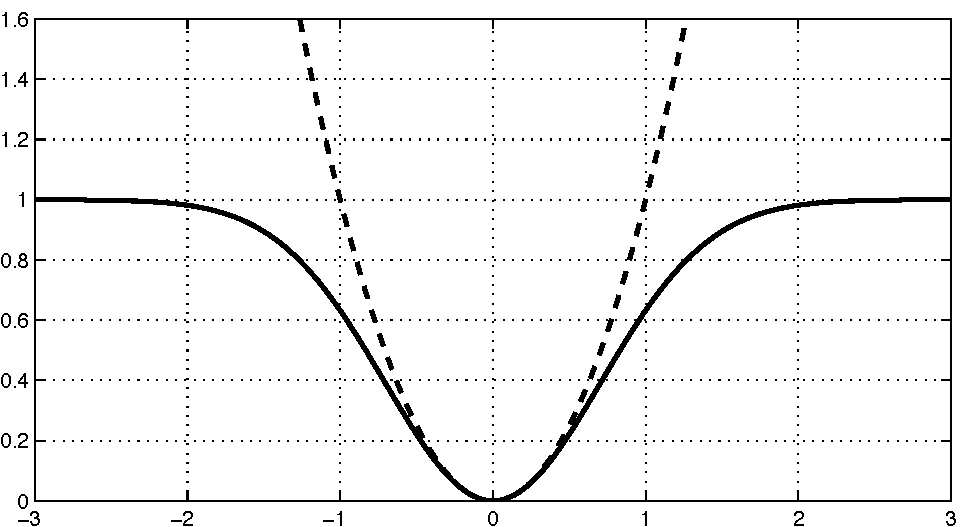
\includegraphics[scale=0.46,clip,trim=0.5cm 0.4cm 0cm 0cm]{figs/gpml/cost_costs.pdf}};
\node[rotate=90] at (-4.25,0) {Stage cost $c(\bz)$};
\node at (-3.8,0.4) {1};
\node at (0,-2.4) {State-action space $\bz$};
\node at (-2.25,-1.5) {\footnotesize Setpoint $\br$};
\path[line] (-1.4,-1.6) -- (-0.3,-1.87);
\end{tikzpicture}
%
\caption{Stage-costs for which the expectation in \Eq{costint} can be evaluated analytically for $\bz_k \sim \cN$. These functions are useful for penalising deviations of the state-action $\bz$ from a given setpoint $\br$. The quadratic is shown by the dashed line and the inverted-Gaussian is shown by the solid.}
\label{fig:cost_costs}
\end{figure}
%-------------------------------------------------------------------------------------------------------------------------------------------


Due to \Ass{moment}, the approximate distribution over state-action at each timestep is Gaussian $\bz_k \sim \cN$. In order to maintain an analytic evaluation problem, we require stage costs in which the expectation
\begin{equation} \label{eqn:costint}
\EE_{\bz_k}\big[c(\bz_k)\big] = \int c(\bz_k)p(\bz_k)\dd\bz_k
\end{equation}
can be evaluated analytically. If we desire to penalise the deviation of the state-action from some given setpoint $\br$ then the standard quadratic and the inverted squared exponential (or ``inverted-Gaussian") stage costs may be considered
\begin{align}
c_{\te{quad}}(\bz) &= \tfrac{1}{2}(\bz - \br)\T\bQ(\bz - \br) \label{eqn:cost_quad} \\
c_{\te{gauss}}(\bz) &= 1 - \exp\Big( - \tfrac{1}{2}(\bz - \br)\T\bQ(\bz-\br)\Big) \label{eqn:cost_gauss}
\end{align}
where $\bQ$ is a positive semi-definite weighting matrix. These are depicted in \Fig{cost_costs} which shows that close to $\br$ these functions are equivalent. The factor of a half is included in the definitions so that the $\bQ$ matrix can be interpreted as the covariance matrix of an unnormalised Gaussian and its elements tuned such that any state-action more than two standard-deviations away from the setpoint will incur a stage cost of approximately one. The inverted-Gaussian stage cost is locally quadratic and can be viewed as a saturated quadratic. The expectations of these costs are given as
\begin{align}
\EE_{\bz}\big[c_{\text{quad}}(\bz)\big] &= \half(\bm - \br)\T\bQ(\bm - \br) + \half\tr(\bS\bQ)
\label{eqn:Equad} \\[-0.3cm]
\EE_{\bz}\big[c_{\text{gauss}}(\bz)\big] &= 1 - \big|\bI + \bS\bQ\big|^{-\sha}
\exp\Big( -\half(\bm - \br)\T
\overbrace{ \bQ^{\sha}(\bI + \bQ^{\sha}\bS\bQ^{\sha})\inv\bQ^{\sha} }^{(\bQ\inv + \bS)\inv}
(\bm - \br)  \Big) \label{eqn:Egauss}
\end{align}
for $\bz \sim \cN(\bm,\bS)$. The use of the inverted-Gaussian stage cost leads to a useful behaviour in the context of probabilistic learning control.







\subsubsection{Natural Exploration-Exploitation}\label{sec:natexp}
The motivation for preferring the inverted-Gaussian stage cost \Eq{cost_gauss} over the conventional quadratic form in the context of learning control will now be outlined. Consider the optimal control problem posed in \Eq{Jcost} in which the initial state is known exactly $\bS_0 = \bO$ and the only source of uncertainty comes from the probabilistic model which is used to capture modelling uncertainty. As part of the offline simulation phase of the learning framework posed in \Sec{modelbased} now consider that the policy has to make a choice between two state-action densities $p_1(\bz)$ and $p_2(\bz)$ as shown in \Fig{exp_far}. If modelling uncertainty was ignored then the policy would favour the state distribution with mean closest to the setpoint $\br$ regardless of the uncertainty associated with the prediction. However, if uncertainty is taken into account, the policy will favour the more uncertain state with mean further from the setpoint since this has more density in the low cost region therefore yields a lower expected cost. 

The converse situation is depicted in \Fig{exp_near} where the probabilistic framework would favour policies that chose the more certain state despite the fact that its mean is further from the setpoint. 
This example illustrates that using a probabilistic model will lead to policies which drive the system into uncertain areas of its state-action space in high cost regions but favour cautious behaviour when close to the setpoint. This ``natural" exploration will aid the model learning process.



%-------------------------------------------------------------------------------------------------------------------------------------------
\begin{figure}[t]
\centering
\tikzstyle{line} = [draw, -latex]
\subfigure[Distributions with means far away from the setpoint]{
\begin{tikzpicture}
\small
\node at (0,0) {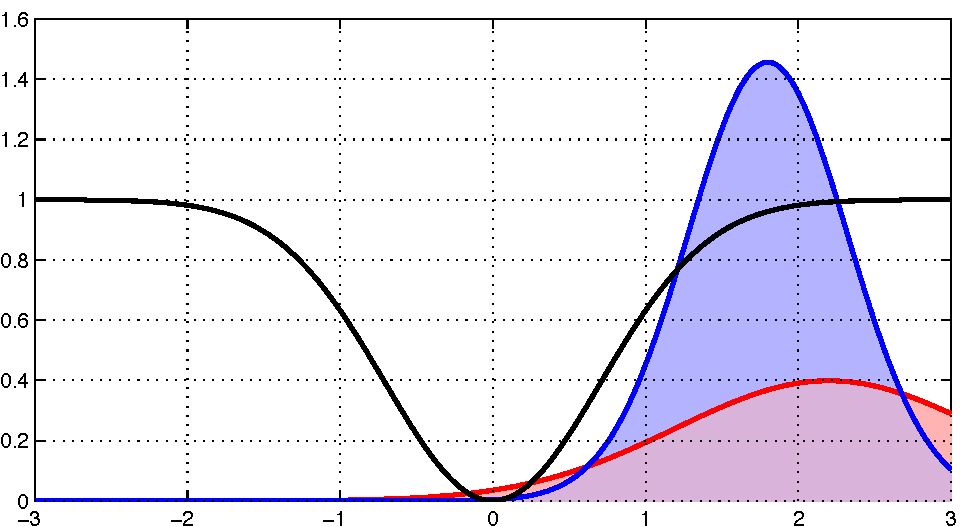
\includegraphics[scale=0.46,clip,trim=0.5cm 0.4cm 0cm 0cm]{figs/gpml/explore_far.pdf}};
\node at (0,-2.4) {State-action space $\bz$};
\node at (-3.0,0.75) {$c(\bz)$};
\node at (2.2,-0.3) {\color{blue}$p_1(\bz)$};
\node at (2.3,-1.55) {\color{red}$p_2(\bz)$};
\end{tikzpicture}
\label{fig:exp_far}
}
\hfill
\subfigure[Distributions with means close to the setpoint]{
\begin{tikzpicture}
\small
\node at (0,0) {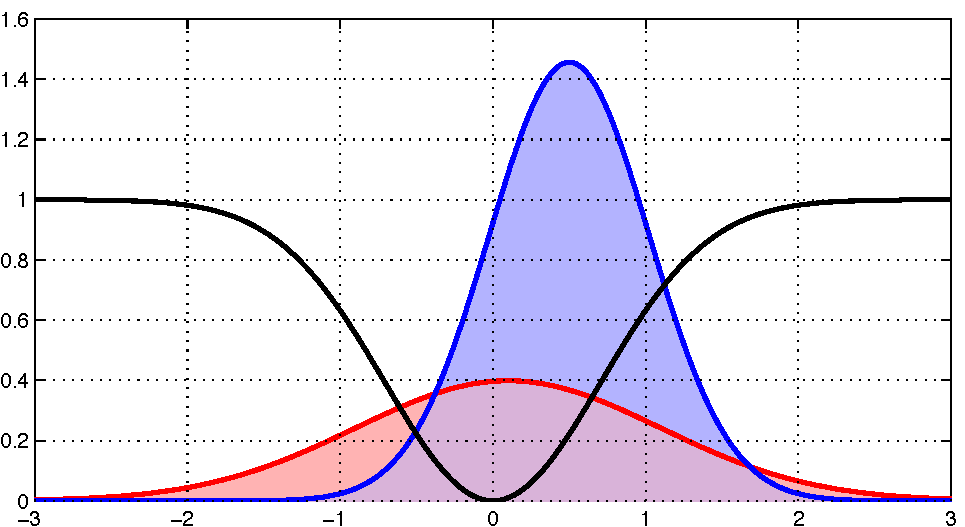
\includegraphics[scale=0.46,clip,trim=0.5cm 0.4cm 0cm 0cm]{figs/gpml/explore_near.pdf}};
\node at (0,-2.4) {State-action space $\bz$};
\node at (-3.0,0.75) {$c(\bz)$};
\node at (0.55,-0.1) {\color{blue}$p_1(\bz)$};
\node at (1.0,-1.7) {\color{red}$p_2(\bz)$};
\end{tikzpicture}
\label{fig:exp_near}
}
\caption{Illustration of how a ``natural" exploration of the state-action space can arise through use of an inverted-Gaussian stage cost. The stage cost is shown as a black line and two distributions over state-action space are shown by the blue and red curves, with the means shown explicitly.}
\end{figure}
%-------------------------------------------------------------------------------------------------------------------------------------------


The standard quadratic cost would not display this behaviour since the covariance of the state-action is always explicitly penalised by the additive term shown in \Eq{Equad}. Therefore the quadratic cost leads only to behaviour which seeks to exploit its current knowledge and not explore. It should be noted that this is not the standard exploration-exploitation tradeoff that appears in the reinforcement learning literature since this behaviour arises from being greedy with respect to a probabilistic model rather than explicitly applying random inputs.






\subsection{Policy Improvement}

Since an analytic approximation to the cost function in \Eq{learn1} is being considered, the gradient of this cost with respect to the policy parameters $\dd J(\bpsi)/\dd\bpsi$ can also be obtained in closed form. This means that we can make efficient use of gradient descent optimisation in order to carry out the improvement step of the simulation phase. The derivatives have the following structure
\begin{align}
\diff{J(\bpsi)}{\bpsi} &= \sum_{k=0}^{H} \diff{\EE_{\bz_k}\big[c(\bz_k)\big]}{\bpsi} 
\label{eqn:Jderiv1}
\end{align}
Due to the Gaussian assumption given in \Ass{moment}, the expectation of the stage cost $\EE_{\bz_k}\big[c(\bz_k)\big]$ is only dependant on the mean and variance of this distribution. Therefore the full derivative can be split up into partial derivatives
\begin{align}
\diff{\EE_{\bz_k}\big[c(\bz_k)\big]}{\bpsi} =
\pdiff{\EE_{\bz_k}\big[c(\bz_k)\big]}{\bm_k} \diff{\bm_k}{\bpsi} +
\pdiff{\EE_{\bz_k}\big[c(\bz_k)\big]}{\bS_k} \diff{\bS_k}{\bpsi}
\end{align}
where $\bm_{k} = \EE_{\bz_{k-1},\bff}[\bz_k|\bpi]$ and $\bS_{k} = \cov_{\bz_{k-1},\bff}[\bz_k|\bpi]$. The dimensions of these derivatives are defined according to the matrix calculus convention outlined in \App{matcal}. The derivatives of the mean and covariance at each step can be calculated in the following recursive manner
\begin{align}
\diff{\bm_k}{\bpsi} &= \pdiff{\bm_k}{\bm_{k-1}}\diff{\bm_{k-1}}{\bpsi} 
+ \pdiff{\bm_k}{\bS_{k-1}}\diff{\bS_{k-1}}{\bpsi} + \pdiff{\bm_k}{\bpsi} \\
\diff{\bS_k}{\bpsi} &= \pdiff{\bS_k}{\bm_{k-1}}\diff{\bm_{k-1}}{\bpsi} 
+ \pdiff{\bS_k}{\bS_{k-1}}\diff{\bS_{k-1}}{\bpsi} + \pdiff{\bS_k}{\bpsi}
\label{eqn:Jderiv2}
\end{align}
for $k \geq 1$ where each partial derivative is dependent on the type of dynamics model and policy structure used. The mean and covariance at $k=0$ can be partitioned as follows
\begin{align*}
\bm_0 &= \bmat{\bm_{\bx_0} \\ \bm_{\bu_0}}, 
&\bS_0 &= \bmat{\bS_{\bx_0} & \bS_{\bx\bu_0} \\ \bS_{\bx\bu_0}\T & \bS_{\bu_0}}
\end{align*}
where $\dd\bm_{\bx_0}/\dd\bpsi = \bO$ and $\dd\bS_{\bx_0}/\dd\bpsi = \bO$ since the initial state distribution is fixed.  The exact form of these derivatives depend on the form of the probabilistic model and the policy used. These calculations are implemented in an iterative fashion using MATLAB and can be found in \App{codeCost} implemented by the function \texttt{value.m}.























\section{State-Action Prediction} \label{sec:xuprediction}


%-------------------------------------------------------------------------------------------------------------------------------------------
\begin{figure}[t]
\centering
\tikzstyle{sum} = [circle, draw, minimum height=1cm]
\tikzstyle{block} = [rectangle, draw, fill=white, text width=7em, text centered, rounded corners, minimum height=4em]
\tikzstyle{line} = [draw, -latex]
%
\begin{tikzpicture}
	\small	
	\node at (-5.4,0.3) {$p(\bx_{k-1},\bu_{k-1})$};
	\node at (0,0.3) {$p(\bx_k)$};
	\node at (5.4,0.3) {$p(\bx_k,\bu_k)$};
	
	\node[block](dyn) at (-2.5,0) {Model \\$p(\bff|\cD,\hyp)$};
	\node[block](pol) at (2.5,0) {Policy \\$\bpi$};
	\path[line] (-6.8,0) -- (dyn.west); \node at (-7.5,0) {. . .};
	\path[line] (dyn.east) -- (pol.west);
	\path[draw] (pol.east) -- (6.8,0); \node at (7.5,0) {. . .};
	
\end{tikzpicture}
\caption{Propagation of uncertainty from a given state-action pair $(\bx_{k-1},\bu_{k-1})$ to the pair at the following timestep $(\bx_k,\bu_k)$ given a distribution over dynamics functions $p(\bff|\cD,\hyp)$ and the control policy $\bpi$.}
\label{fig:propxu}
\end{figure}
%-------------------------------------------------------------------------------------------------------------------------------------------

\subsection{Propagating Uncertainty}
Attention is now turned to the problem of inferring the assumed Gaussian distribution over state-action space $p(\bz_k)$ given the distribution at the previous timestep $p(\bz_{k-1}) \sim \cN$. This can then be cascaded in order to build up a distribution over the full trajectory $p(\btau)$. It would be useful to treat this problem in two stages as shown in \Fig{propxu}. First, find the distribution $p(\bx_k)$ using the probabilistic dynamics model $p(\bff|\cD,\hyp)$. Then find the joint distribution $p(\bx_k,\bu_k)$ using the policy $\bpi$. In order to do this, a tighter assumption is made:

\begin{ass}\label{ass:gauss}
Given $p(\bz_{k-1})$ is Gaussian, the resulting distribution of the next state-action $p(\bz_k)$ is replaced by the Gaussian distribution
\begin{equation*}
\bmat{\bx_k \\ \bu_k} \sim \cN\left(
\bmat{\EE_{\bz_{k-1},\bff}[\bx_k] \\ \EE_{\bchi_k}[\bu_k|\bpi]},
\bmat{\cov_{\bz_{k-1},\bff}[\bx_k] & \cov_{\bchi_k}[\bchi_k,\bu_k|\bpi] \\
\cov_{\bchi_k}[\bu_k,\bchi_k|\bpi] & \cov_{\bchi_k}[\bu_k|\bpi]}
\right)
\end{equation*}
where $p(\bchi_k)$ is the moment matched approximation of the real distribution $p(\bx_k)$.
%Given $p(\bz_{k-1}) \sim \cN$, the distribution of the next state $p(\bx_k)$ is Gaussian with mean $\EE_{\bz_{k-1},\bff}[\bx_k]$ and covariance $\cov_{\bz_{k-1},\bff}[\bx_k]$. Additionally, the joint distribution $p(\bz_{k-1},\bx_k) \sim \cN$ is also Gaussian with cross covariance $\cov_{\bz_{k-1},\bff}[\bz_{k-1}, \bx_k|\bpi]$.
\end{ass}

Note that \Ass{moment} uses the real distribution $p(\bx_k)$ as the input to the control policy whereas \Ass{gauss} uses the moment matched approximation $p(\bchi_k)$. From now on, no distinction will be made between the real distribution $p(\bx)$ and its approximation $p(\bchi)$.
%Therefore, given Assumptions \ref{ass:moment} and \ref{ass:gauss} the distribution of $\bz_k$ given $\bz_{k-1}$ can be partitioned as
%\begin{equation}
%\bmat{\bx_k \\ \bu_k} \sim \cN\left(
%\bmat{\EE_{\bz_{k-1},\bff}[\bx_k] \\ \EE_{\bx_k}[\bu_k|\bpi]},
%\bmat{\cov_{\bz_{k-1},\bff}[\bx_k] & \cov_{\bx_k}[\bx_k,\bu_k|\bpi] \\
%\cov_{\bx_k}[\bu_k,\bx_k|\bpi] & \cov_{\bx_k}[\bu_k|\bpi]}
%\right)
%\label{eqn:jointgauss}
%\end{equation}






\subsection{Gaussian Approximation Schemes}
The use of the moment matching scheme given in Assumptions \ref{ass:moment} and \ref{ass:gauss} will now be motivated. For now, consider the propagation of uncertainty from the input $\bz \sim \cN(\bm,\bS)$ through a distribution over functions $p(\bff)$ to the next state $\bff(\bz)$. In this case we assume that the probabilistic model returns a Gaussian distribution when queried at a deterministic input. This is the first step shown in \Fig{propxu}. There are a number of methods available for approximating the real distribution $p\big(\bff(\bz)\big)$ with a Gaussian $\cN(\bm_*,\bS_*)$. We shall briefly introduce a number of these methods now
%
\begin{enumerate}
\item {\bf Taylor Series Expansions.} Approximate the dynamics $p(\bff)$ with a finite Taylor series expansion of the real nonlinear equations about the input mean $\bm$. Then for a first order expansion for example we have 
\begin{align*}
\bm_* &= \EE_{\bff}[\bff(\bm)] 
&\bS_* &= \big( \partial\EE_{\bff}[\bff(\bm)]/\partial\bm \big)^2 + \cov_{\bff}[\bff(\bm)]
\end{align*}
This is equivalent to taking linearisations, which is the method that is used in the prediction step of the Extended Kalman Filter (EKF). See Chapter 8 of \cite{AnMo79} for more information on the EKF.
%
\item {\bf Unscented Transformation.} Instead of making assumptions about the structural nature of the dynamics model or policy, the unscented transformation takes a finite number of (weighted) ``sigma-points" $\cS = \{\hat\bz_{1} \dots \hat\bz_{S}\}$ with the same second-order statistics as $p(\bz)$. Mathematically
$\EE_{\bz}[\bz] = \sum_{s=1}^S W_s\hat\bz_{s}$ and $\cov_{\bz}[\bz] = \sum_{s=1}^S W_s(\hat\bz_{s}-\EE_{\bz}[\bz])(\hat\bz_{s}-\EE_{\bz}[\bz])\T$
where $\sum_{s=1}^S W_s=1$, $W_s > 0$. It then maps them through the mean of the probabilistic dynamics model to obtain the transformed set $\EE_{\bff}[\bff(\cS)] = \{\EE_{\bff}[\bff(\hat\bz_{1})] \dots \EE_{\bff}[\bff(\hat\bz_{S})]\}$. The mean and covariance are then set to that of the (weighted) statistics of the transformed data set
\begin{align*}
\bm_* &= \sum_{s=1}^S W_s\EE_{\bff}[\bff(\hat\bz_{s})] 
&\bS_* &= \sum_{s=1}^S W_s\big(\EE_{\bff}[\bff(\hat\bz_{s})]-\bm_*\big)\big(\EE_{\bff}[\bff(\hat\bz_{s})]-\bm_*\big)\T
+ \cov_{\bff}[\bff(\bm)]
\end{align*}
respectively to give an unbiased prediction. This method was proposed as the prediction step of the Unscented Kalman Filter (UKF) of \cite{JU97}.
%
\item {\bf Exact Moment Matching.} In situations where they are possible to obtain, the moment matching approximation finds the exact mean and covariance 
\begin{align*}
\bm_* &= \EE_{\bz,\bff}[\bff(\bz)]
& \bS_* &= \cov_{\bz,\bff}[\bff(\bz)]
\end{align*}
of the actual distribution $p\big(\bff(\bz)\big)$. To complete the filtering parallel of the previous two examples, the moment matching technique is used in the prediction step of an Assumed Density Filter (ADF). See Chapter 12 of \cite{May82} for more information on the ADF.
\end{enumerate}


%-------------------------------------------------------------------------------------------------------------------------------------------
\begin{figure*}
\centering
\footnotesize
\subfigure[Linear approximation. Linearisations of the function about the state-action mean $\EE{[\bz]}$ are shown.]{
\tikzstyle{line} = [draw, -latex]
\begin{tikzpicture}
\node at (-7.4,-3) {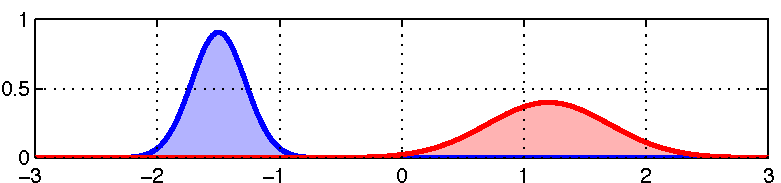
\includegraphics[scale=0.6, clip, trim=0.5cm 0.4cm 0cm 0cm]{figs/gpml/propLIN_1.pdf}};
\node at (-7.4,0) {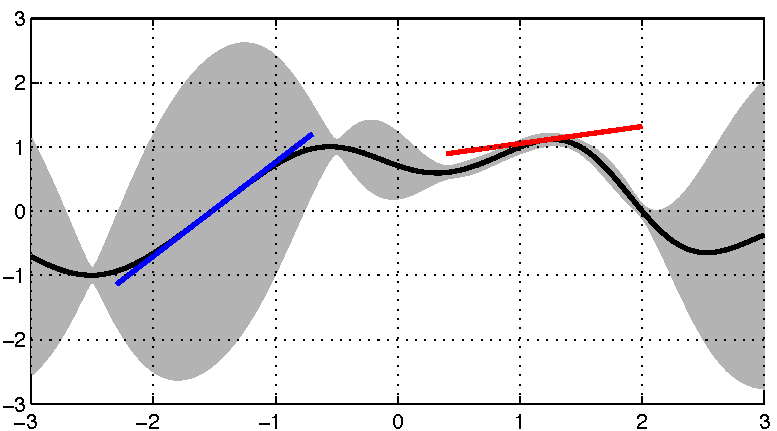
\includegraphics[scale=0.6, clip, trim=0.5cm 0.4cm 0cm 0cm]{figs/gpml/propLIN_2.pdf}};
\node at (0,0) {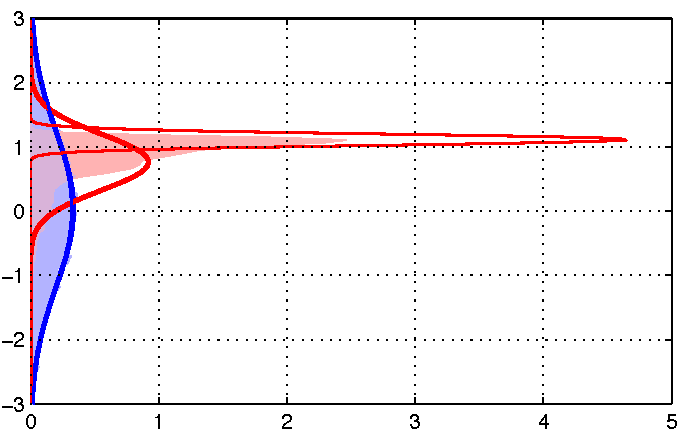
\includegraphics[scale=0.6, clip, trim=0.5cm 0.4cm 0cm 0cm]{figs/gpml/propLIN_3.pdf}};

\node at (-8.3,-3) {\color{blue} $p_1(\bz)$};
\node at (-5,-3) {\color{red} $p_2(\bz)$};
\node[rotate=90] at (-11.5,0) {Function distribution};
\node at (-10.5,1.55) {$p(\bff)$};
\node at (-2.4,-1.1) {\color{blue} $q_1\big(\bff(\bz)\big)$};
\node at (-1.3,0.2) {\color{red} $q_2\big(\bff(\bz)\big)$};

\draw[rounded corners,fill=white] (-0.5,-1.85) rectangle (3,-0.25);
\node[fill=blue!30,circle,minimum height=0.33cm] at (-0.2,-0.65) {};
\node[fill=red!30,circle,minimum height=0.33cm] at (0.15,-0.65) {};
\draw[very thick,blue] (-0.35,-1.08) -- (-0.05,-1.08); \draw[very thick,red] (0.0,-1.08) -- (0.3,-1.08);
\draw[thin,blue] (-0.35,-1.48) -- (-0.05,-1.48); \draw[thin,red] (0.0,-1.48) -- (0.3,-1.48);
\node[anchor=west] at (0.35,-0.65) {Monte Carlo};
\node[anchor=west] at (0.35,-1.05) {Exact Moments};
\node[anchor=west] at (0.35,-1.45) {\bf Linearised};

\end{tikzpicture}
\label{fig:propLinUnsA}
}
%
\subfigure[Unscented transformation. Sigma points $\cS$ along with their projections $\bff(\cS)$ and weights $W$ are shown.]{
\tikzstyle{line} = [draw, -latex]
\begin{tikzpicture}
\node at (-7.4,-3) {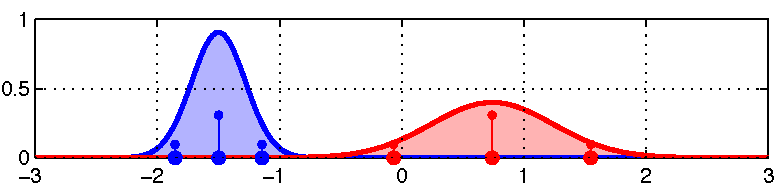
\includegraphics[scale=0.6, clip, trim=0.5cm 0.3cm 0cm 0cm]{figs/gpml/propUNS_1.pdf}};
\node at (-7.4,0) {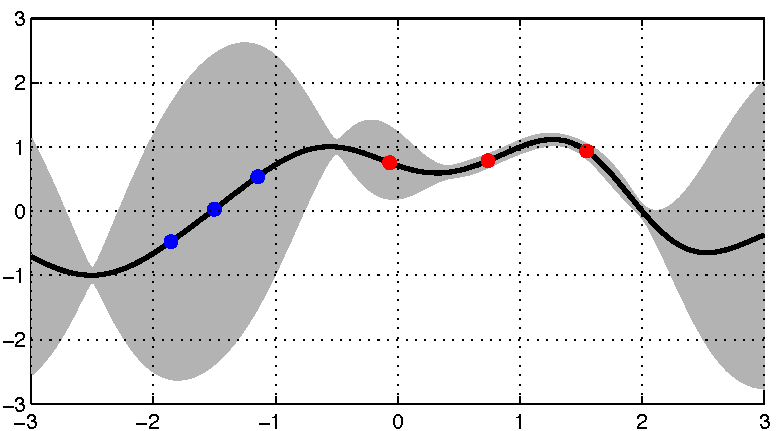
\includegraphics[scale=0.6, clip, trim=0.5cm 0.4cm 0cm 0cm]{figs/gpml/propUNS_2.pdf}};
\node at (0,0) {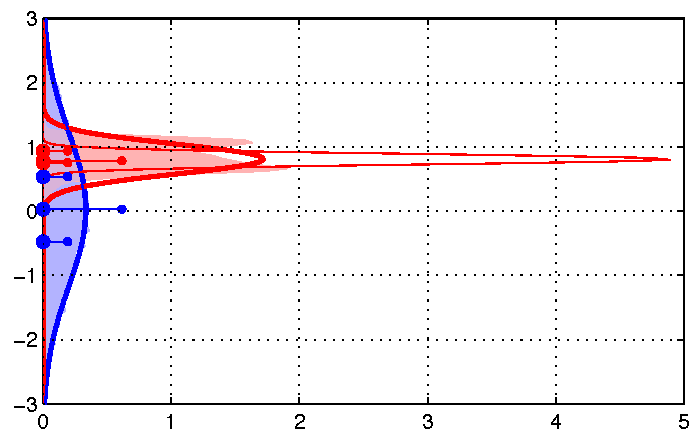
\includegraphics[scale=0.6, clip, trim=0.6cm 0.4cm 0cm 0cm]{figs/gpml/propUNS_3.pdf}};

\node at (-8.3,-3) {\color{blue} $p_3(\bz)$};
\node at (-5,-3) {\color{red} $p_4(\bz)$};
\node[rotate=90] at (-11.5,0) {Function distribution};
\node at (-10.5,1.55) {$p(\bff)$};
\node at (-2.4,-1.1) {\color{blue} $q_3\big(\bff(\bz)\big)$};
\node at (-1.2,0.0) {\color{red} $q_4\big(\bff(\bz)\big)$};

\draw[rounded corners,fill=white] (-0.5,-1.85) rectangle (3,-0.25);
\node[fill=blue!30,circle,minimum height=0.33cm] at (-0.2,-0.65) {};
\node[fill=red!30,circle,minimum height=0.33cm] at (0.15,-0.65) {};
\draw[very thick,blue] (-0.35,-1.08) -- (-0.05,-1.08); \draw[very thick,red] (0.0,-1.08) -- (0.3,-1.08);
\draw[thin,blue] (-0.35,-1.48) -- (-0.05,-1.48); \draw[thin,red] (0.0,-1.48) -- (0.3,-1.48);
\node[anchor=west] at (0.35,-0.65) {Monte Carlo};
\node[anchor=west] at (0.35,-1.05) {Exact Moments};
\node[anchor=west] at (0.35,-1.45) {\bf Unscented};
\end{tikzpicture}
\label{fig:propLinUnsB}
}
\caption{Propagation of uncertainty through a deterministic mapping $\bff$ using linearisation, the unscented transformation and exact moment matching. The lower plots show two distributions over $\bz$. The central plot shows the stochastic function $\bff$ with mean shown by the solid line and the 2$\sigma$ uncertainty region in gray. The right hand plot shows the true output distributions (obtained by sampling) and the various approximation schemes. Fig.$\!$ (a) is an example of the degeneracy of the linearised approximation and Fig.$\!$ (b) shows the degeneracy of the unscented transform.}
\label{fig:propLinUns}
\end{figure*}
%-------------------------------------------------------------------------------------------------------------------------------------------


%-------------------------------------------------------------------------------------------------------------------------------------------
%\begin{figure}[t]
%\centering
%\subfigure[Linear approximation. Linearisations of the function about the state-action mean $\EE{[\bz]}$ are shown.]{
%\tikzstyle{line} = [draw, -latex]
%\begin{tikzpicture}
%\scriptsize
%\node at (0,0) {\includegraphics[width=0.45\textwidth, clip, trim=1cm 0cm 0cm 0cm]{figs/gpml/propLin.pdf}};
%\draw[fill=white,white] (1.4,-2.1) rectangle (1.6,-0.8);
%\path[line] (-3.58,-2.13) -- (-3.58,-1.0); \path[line] (-3.68,-2.03) -- (1,-2.03); % bottom
%\path[line] (-3.58,-0.9) -- (-3.58,2.2); \path[line] (-3.68,-0.8) -- (1,-0.8); % middle
%\path[line] (1.47,-0.9) -- (1.47,2.2); \path[line] (1.37,-0.8) -- (3.5,-0.8); % right
%\node at (0.7,-0.55) {$\bz$}; \node at (-3.17,-1.2) {$p(\bz)$};
%\node at (-3.2,1.95) {$\bff(\bz)$}; %\node at (0.8,-1.0) {$\bz$};
%\node at (3.0,-0.5) {$p\big(\bff(\bz)\big)$};
%\end{tikzpicture}
%\label{fig:propLinUnsA}
%}
%
%\hfill
%
%\subfigure[Unscented transformation. Sigma points $\cS$ along with their projections $\bff(\cS)$ and weights $W$ are shown.]{
%\tikzstyle{line} = [draw, -latex]
%\begin{tikzpicture}
%\scriptsize
%\node at (0,0) {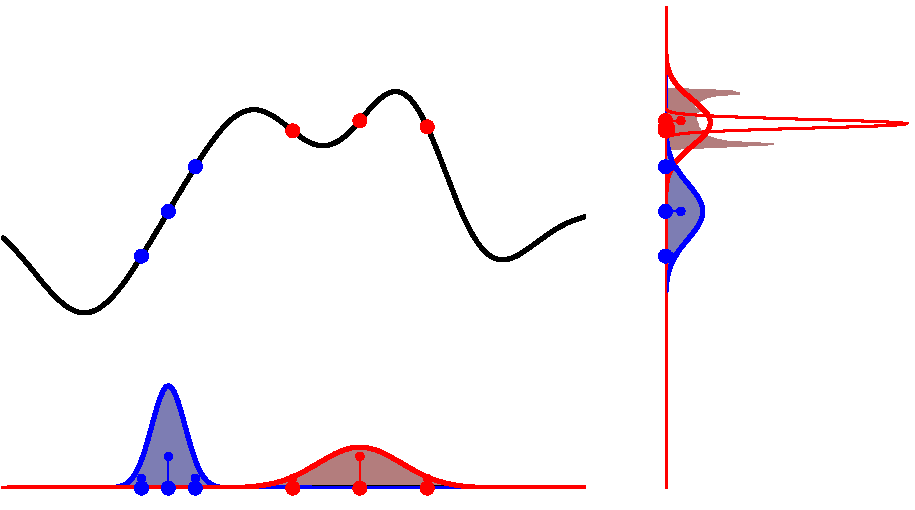
\includegraphics[width=0.45\textwidth, clip, trim=1cm 0.2cm 0cm 0cm]{figs/gpml/propUns.pdf}};
%\draw[fill=white,white] (1.4,-2.1) rectangle (1.6,-0.8);
%\path[line] (-3.58,-2.115) -- (-3.58,-1.0); \path[line] (-3.68,-2.015) -- (1,-2.015); % bottom
%\path[line] (-3.58,-0.9) -- (-3.58,2.2); \path[line] (-3.68,-0.8) -- (1,-0.8); % middle
%\path[line] (1.5,-0.9) -- (1.5,2.2); \path[line] (1.4,-0.8) -- (3.5,-0.8); % right
%\node at (0.7,-0.55) {$\bz$}; \node at (-3.17,-1.2) {$p(\bz)$};
%\node at (-3.2,1.95) {$\bff(\bz)$}; %\node at (0.8,-1.0) {$\bz$};
%\node at (3.0,-0.5) {$p\big(\bff(\bz)\big)$};
%\end{tikzpicture}
%\label{fig:propLinUnsB}
%}
%\caption{Propagation of uncertainty through a deterministic mapping $\bff$ using linearisation about the mean of the state-action distribution, the unscented transformation and an exact moment matching approach. The lower plot shows two input distributions over $\bz$. The central plot shows the mapping underlying function $\bff$. The right hand plot shows Monte-Carlo approximations of the real output distributions (shaded), and moment matched (thick solid) Gaussian approximations. Plot (a) shows two examples of the linearised approximation (thin solid) where the red example is approaching degeneracy. Plot (b) shows two examples of the unscented transformation (thin solid) where the red example is approaching degeneracy.}
%\label{fig:propLinUns}
%\end{figure}
%-------------------------------------------------------------------------------------------------------------------------------------------




%
Both the Taylor series expansion and the unscented transformation methods can potentially suffer from degeneracy as demonstrated in \Fig{propLinUns}. In the cases depicted by the blue distributions the function $\bff$ is close to linear in the region where the distribution has high density and therefore all methods make good approximations to the actual distribution. An example of the degeneracy of the linear approximation is shown by the red plot in \Fig{propLinUnsA} where the gradient approaches zero and the output distribution approaches the delta distribution and ignores much of the mass of the real output distribution. Similarly, the potential degeneracy of the unscented transformation is demonstrated in the red case shown in \Fig{propLinUnsB}. A further example is given in \cite{DTHH12}. 

The moment matching approach does not suffer from degeneracy for obvious reasons. We further note that the moment matching approach is, in a sense, a conservative approximation. In order to appreciate this, consider the 
Kullback-Leibler (KL) divergence $\mathrm{KL}\big(q || p\big)$ of the underlying distribution $p$ with respect to some Gaussian distribution $q$. We can prove that the Gaussian which minimises this divergence is the moment matched solution. For details of this proof see \App{KLdiv}. 
%
The nature of the KL divergence ensures that the approximate distribution $q$ is non-negligible where the real distribution $p$ is non-negligible, but not the other way around. In this sense the predictions will be conservative.

The advantage of using a Taylor series or unscented transformation based method is that they can be applied to a broader class of systems whereas the moment matching assumption is more restrictive. However, since a very useful set of models is amenable to the moment matching approach this was the method that has been adopted in this thesis.



\subsection{Modelling Uncertainty}
In a learning context it is important to treat modelling uncertainty in a rigorous manner. This is readily handled in a Bayesian framework. Given a parametric representation of the dynamics consisting of a linear sum of appropriate basis functions the Bayesian framework provides a way of making predictions based on a prior distribution over parameters and an observed data set.


% Further, it would be preferable not to impose a full parametric structure on the form of the dynamics that are to be modelled as this process can often be based on oversimplifying assumptions. Rather, it would be good to make predictions based on observed data and some higher level assumptions regarding the structure of the dynamics, such as smoothness or some intrinsic length-scale. These issues are well handled by the nonparametric probabilistic modelling framework of Gaussian processes.
















\section{Bayesian Modelling} \label{sec:bayesmodelling}%%%%%%%%%%%%%%%%%%%%%%%%%%%%%%%%

\subsection{Problem Outline} \label{sec:bayesproblem}
This section considers the problem of finding a probabilistic model $p(\bff|\cD, \hyp)$ defining a distribution over the function space, given some training data set $\cD$ and hyperparameters $\hyp$ and using this model to make predictions. This problem can be addressed by a Bayesian method known as Gaussian Processes (GPs). A Gaussian process  is defined by \cite{RaWi06} in \Def{GP}.

\begin{defin}[Gaussian process] \label{def:GP}
A collection of random variables, any finite number of which have a joint Gaussian distribution.
\end{defin}
%
Informally speaking, GPs are a means of placing a prior over a space of functions $p(\bff|\hyp)$ from which samples can be drawn, an extension of the idea of multivariate Gaussian distributions to infinitely long vectors, or functions. Once training data has been observed, this can be updated to a posterior distribution $p(\bff|\cD,\hyp)$ which is the probabilistic model required by the learning framework outlined in \Sec{learnover}.
%
Given a deterministic input $\bz$, GPs provide a predictive Gaussian distribution over possible next states with mean $\EE_{\bff}[\bff(\bz)|\bz,\cD]$ and covariance $\cov_{\bff}[\bff(\bz)|\bz,\cD]$. Explicit dependence on the hyperparameters $\hyp$ will be dropped from now on for clarity. However, from \Sec{xuprediction}, making predictions with respect to uncertain $\bz \sim \cN$ is required for the moment matching framework. In other words, making predictions of the mean $\EE_{\bz,\bff}[\bff(\bz)|\cD]$ and covariance $\cov_{\bz,\bff}[\bff(\bz)|\cD]$.



%In order to motivate their relevance in this context, a parametric approach to modelling will be considered which will to a full nonparametric framework. First, the form of the training data set $\cD$ must be considered.

Now the exact form of the training data set $\cD$ will be discussed. Data will be given in the form of $n$ state-actions and next-state pairs
\begin{align}
\bZ &= \bmat{ \bx_{k_1}\T & \bu_{k_1}\T \\ \vdots & \vdots \\ \bx_{k_n}\T & \bu_{k_n}\T} \in \RR^{n \times D} &\text{and}
&& \bY &= \bmat{ \bx_{k_1+1}\T \\ \vdots \\ \bx_{k_n+1}\T } \in \RR^{n\times E} \label{eqn:cZY}
\end{align}
for $-\infty < k_1 < \dots < k_n < 0$ not necessarily sampled consecutively. For the purposes of the following discussion, state-action pairs are referred to as ``inputs" and the next-states are referred to as ``outputs". Now, an important issue arises here. In reality all of these measurements will be corrupted by noise, normally assumed to be additive Gaussian noise. However, the GP framework assumes that only the outputs $\bY$ are corrupted by additive noise $\be \sim \cN(\bO, \bS_{\be})$ with diagonal covariance $\bS_{\be}$ and uncorrelated between timesteps but the inputs are noise free. The GP approach to a fully noisy data set will be discussed later, but for now this assumption will be made. Therefore, the noisy output measurements will be referred to by $\bY$, while the noise-free set is referred to by the matrix $\bF$.
%where $\by = \bx + \be$ are state measurements corrupted by noise  The underlying values of the next-states are stored in the matrix $\bF = \big[\bx_{t_1+1} \dots \bx_{t_n+1} \big]$. In this framework it is assumed that the underlying state is available in order to form the $\bZ$ matrix. %This assumption may of course be unrealistic and is addressed formally by \cite{MR11} who consider the case of noisy input values in a Gaussian process framework. 

It is worthy of note that the following presentation of Gaussian process theory is novel in the sense that we deal with the multivariate case from the very outset. Most textbooks and presentations of the fundamental theory talk about the multivariate case as an afterthought.







\subsection{Parametric Approach}
\subsubsection{Prior}
The linear parametric approach assumes that the unknown function $\bff: \RR^D \rightarrow \RR^E$ belongs to the set of functions parameterised by
\begin{equation}
\bff(\bz) = \bPh(\bz)\T \bw    \label{eqn:param}
\end{equation}
where $\bw \in \RR^{P}$ is a vector of weights and the feature matrix $\bPh(\bz) \in \RR^{P\times E}$ is made up of a number of basis functions. Note that the feature matrix is often of a form such that there are no cross correlations between output dimensions through common weights. In other words $\bPh(\bz) = \bI \otimes \bph(\bz)$. The feature matrix is defined to handle matrix inputs by defining the following convention
\begin{align}
\bPh(\bZ) &:= \bmat{ \Phi[:,1](\bZ) & \dots & \Phi[:,E](\bZ) } \in \RR^{P \times En}
\label{eqn:Phi1} \\
\Phi[:,i](\bZ) &:= \bmat{ \Phi[:,i](\bz_{k_1}) & \dots & \Phi[:,i](\bz_{k_n}) } \in \RR^{P \times n}
\label{eqn:Phi2}
\end{align}
 where $\Phi[:,i](\bz)$ is the $i\tth$ column of $\bPh(\bz)$. Note that the standard linear dynamics model $\bff(\bz) = \bA\bx +\bB\bu$ falls under this model class by setting $\bPh(\bz) = \bI \otimes \bz$ and $\bw = \vect\big([\bA \;\bB]\T\big)$. In a Bayesian framework a prior distribution is placed over the unknown parameter space $p(\bw|\hyp) = \cN(\bet,\bOm)$ which is defined in terms of the hyperparameters $\hyp = \{\bet,\bOm\}$ and represents any prior knowledge regarding their relationship. 

This prior over parameters leads to a prior over the space of functions $p(\bff|\hyp)$ which satisfies the definition of a Gaussian process. The GP is parameterised by a \textit{mean function} and \textit{covariance function} (or \textit{kernel}) defined to be
\begin{align}
\bmm(\bz) &:= \EE_{\bw}\big[\bff(\bz)\big] &&
\!\!\!\!\!\!\!\!\!\!\!\!\!\!\!\!\!\!\!\!\!\!\!\!\!\!\!\!\!\!\!\!\!\!\!\!\!\!\!\!\!\!\!\!\!\!\!\!\!\!\!\!\!\!\!\!\!\!\!\!
= \bPh(\bz)\T\bet \\
\bK(\bz,\tilde\bz) &:= \cov_{\bw}\big[\bff(\bz), \bff(\tilde\bz)\big] &&
\!\!\!\!\!\!\!\!\!\!\!\!\!\!\!\!\!\!\!\!\!\!\!\!\!\!\!\!\!\!\!\!\!\!\!\!\!\!\!\!\!\!\!\!\!\!\!\!\!\!\!\!\!\!\!\!\!\!\!\!
= \bPh(\bz)\T \bOm \bPh(\tilde\bz) \label{eqn:covfunc}
\end{align}
respectively. These functions are also defined to take matrix inputs with dimensions determined through the way in which matrix inputs are handled by $\bPh$. For example, if $\bPh(\bz) = \bI \otimes \bph(\bz)$ the covariance matrix $\bK(\bZ,\bZ)$ would be block diagonal, with one block per output dimension. For notational convenience we shall now define $\bK_{nn}:=\bK(\bZ,\bZ)$. The covariance function can also accept a single input by letting $\bK(\bz) := \bK(\bz,\bz)$. Zero mean priors $\bet = \bO$ shall be considered for the remainder of this discussion in order to keep the notation uncluttered, however extension to $\bet \neq \bO$ is trivial.





%-------------------------------------------------------------------------------------------------------------------------------------------
\begin{figure}[t]
\centering
\small
\subfigure[Samples from the prior $p(\bff|\hyp)$.]{
\tikzstyle{line} = [draw, -latex]
\begin{tikzpicture}
	\node at (0,0) {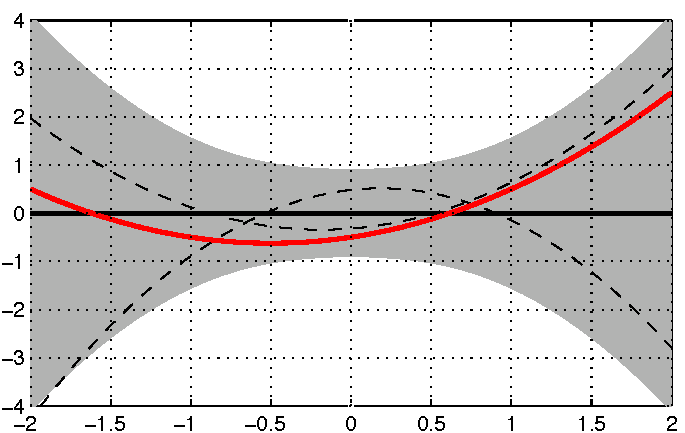
\includegraphics[scale=0.67, clip, trim = 0.5cm 0.45cm 0.2cm 0cm]{figs/gpml/priorRBF.pdf}};
	\node at (3.2,-2.05) {$\bz$};
	\node at (-3.2,1.75) {$\bff(\bz)$};
\end{tikzpicture}
}
\hfill
\subfigure[Samples from the posterior $p(\bff|\cD,\hyp)$.]{
\tikzstyle{line} = [draw, -latex]
\begin{tikzpicture}
	\node at (0,0) {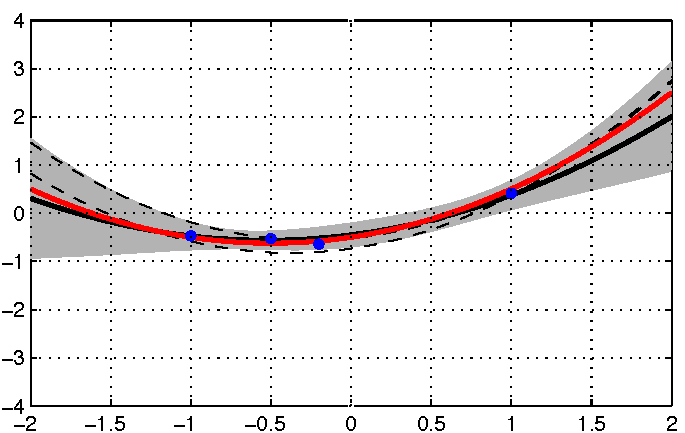
\includegraphics[scale=0.67, clip, trim = 0.5cm 0.45cm 0.2cm 0cm]{figs/gpml/postRBF.pdf}};
	\node at (3.2,-2.05) {$\bz$};
	\node at (-3.2,1.75) {$\bff(\bz)$};
\end{tikzpicture}
}
\caption{Samples from a prior and posterior distribution over quadratic functions $\bff(\bz) = \bPh(\bz)^\top\bw$ where $\bph(\bz) = \big[1; \bz; \vect(\bz\bz^\top)\big]$ with prior Gaussian distribution over the weights $p(\bw|\hyp) = \cN(\bO,\bOm)$.  The red, black and dashed lines show the underlying function $\bff$, mean of the distribution over functions (prior $\bmm$ and posterior $\bmm_+$) and sampled functions respectively. The grey regions denote two standard deviations, or 95\% confidence region, of the distribution. Training data is shown as blue dots on the posterior plot.}
\label{fig:linearprior}
\end{figure}
%-------------------------------------------------------------------------------------------------------------------------------------------




\subsubsection{Posterior}
The posterior over parameters given the observed data set $\cD$ is computed using Bayes' rule
\begin{equation}
p(\bw|\cD,\hyp) = \frac{p(\bY|\bw,\bZ,\hyp)}{p(\bY|\bZ,\hyp)} p(\bw|\hyp)
\end{equation}
where $p(\bY|\bw,\bZ,\hyp)$ is the \textit{likelihood} of the data given the parameters and $p(\bY|\bZ,\hyp)$ is the \textit{marginal likelihood} (or \textit{evidence}) since it is the likelihood of the data marginalised over the parameters $ p(\bY|\bZ,\hyp) = \int p(\bY|\bw,\bZ,\hyp) p(\bw|\hyp) \dd\bw$. Note that the prior over parameters is independent of the training input set therefore $p(\bw|\hyp) = p(\bw|\bZ,\hyp)$.
%
Given that the likelihood and the prior are simply multivariate Gaussians, their product can be calculated analytically as
\begin{align}
p(\bw|\cD,\hyp) &\propto  p(\bY|\bw,\bZ,\hyp) p(\bw|\hyp) 
= \cN\Big( \bPh(\bZ)\T \bw, \bS_{\be}\otimes\bI \Big)  \cN(\bet,\bOm)
\end{align}
where the product is an unnormalised Gaussian which can be found using the identity given in \App{gauss}. It is assumed that the additive noise covariance $\bS_{\be}$ is also a hyperparameter to be inferred. By normalising this product, the posterior over parameter space is given in closed form as $p(\bw|\cD,\hyp) = \cN(\bet_+, \bOm_+)$ with mean and covariance
\begin{align}
\bet_+ &= \Big( \bOm^{-1} + \bPh(\bZ)( \bS_{\be}\otimes\bI)^{-1}\bPh(\bZ)\T \Big)^{-1}\bPh(\bZ)( \bS_{\be}\otimes\bI)^{-1}\vec\bY \label{eqn:parampostM}\\
\bOm_+ &= \Big( \bOm^{-1} + \bPh(\bZ)( \bS_{\be}\otimes\bI)^{-1}\bPh(\bZ)\T \Big)^{-1} \label{eqn:parampostV}
\end{align}
Since the distribution is Gaussian, the mean $\bet_+ = \EE[\bw|\cD,\hyp]$ is the Maximum A Posteriori (MAP) estimate of the parameters $\bw$.  It follows that the posterior distribution over function space $\bff|\cD \sim \mathcal{GP}\big(\bmm_+, \bK_+\big)$ is also a Gaussian process with mean function and covariance function
\begin{align}
\bmm_+(\bz) &= \bPh(\bz)\T\bet_+ \label{eqn:rbfM} \\
\bK_+(\bz,\tilde\bz) &= \bPh(\bz)\T \bOm_+ \bPh(\tilde\bz) \label{eqn:rbfV}
\end{align}
An example of sampling from the prior and posterior of a single-input single-output quadratic function is shown in \Fig{linearprior}. Prediction is then achieved simply as $p\big(\bff(\bz)|\bz,\cD,\hyp\big) = \cN\big(\bmm_+(\bz), \bK_+(\bz) \big)$.

It is instructive to note that as the prior becomes ``flat", $\bOm =\omega\bI$ as $\omega\rightarrow \infty$, the posterior mean prediction tends to $\bet_+ \rightarrow \big(\bPh(\bZ)\bPh(\bZ)\T\big)^{-1}\bPh(\bZ)\vec\bY$. This is the solution of the linear least squares problem $\bPh(\bZ)\T\bp = \vec\bY$. A flat prior implies that the MAP estimate is the same as the Maximum Likelihood estimate since $p(\bw|\cD,\hyp) \propto p(\bY|\bw,\bZ,\hyp)$.






\subsubsection{Kernel Trick} 
The expressions for the posterior mean and covariance in \Eqs{rbfM}{rbfV} can be manipulated into an equivalent form given in \Theo{kerneltrick}. This is a well known result in the Machine Learning community and is based on \textit{Mercer's Theorem}, see \cite{Mer1909}. As will be shown in the following section, these are actually the predictive equations for a Gaussian process. 

\begin{theo}[Kernel Trick] \label{theo:kerneltrick}
%
The expressions for the posterior mean and covariance function in \Eqs{rbfM}{rbfV} are equivalent to 
\begin{align}
\bmm_{+}(\bz) &= \bK(\bz,\bZ) \Big(\bK_{nn}+\bS_{\be}\otimes\bI\Big)^{-1} \vec\bY  \label{eqn:rbfM2} \\
\bK_{+}(\bz,\tilde\bz) &= \bK(\bz,\tilde\bz) - 
\bK(\bz,\bZ) \Big(\bK_{nn}+\bS_{\be}\otimes\bI\Big)^{-1}\bK(\bZ,\tilde\bz) \label{eqn:rbfV2}
\end{align}
where the kernel matrices $\bK$ consist of inner products of the feature matrix $\bPh$ with respect to the prior covariance $\bOm$ as defined in \Eq{covfunc}.
%
\spa \end{theo}

\begin{proof}
Let $\bA = \bOm$, $\bB = \bS_{\be}\otimes\bI$ and $\bC = \bPh(\bZ)$.  Then the parameter mean $\bet_+$ from \Eq{parampostM} can be written as
\begin{align*}
\bet_+ &= \big( \bA^{-1} + \bC\bB\inv\bC\T \big)^{-1} \bC\bB\inv \vec\bY \\
&= \bA\bC \big(  \bC\T\bA\bC + \bB \big)^{-1} \vec\bY \\
&= \bOm\bPh(\bZ) \Big( \bPh(\bZ)\T\bOm\bPh(\bZ) + \bS_{\be}\otimes\bI \Big)^{-1}  \vec\bY
\end{align*}
which follows from a variant of the matrix inversion lemma\footnote{$(\bP\inv + \bR\bQ\inv\bR\T)\inv\bR\bQ\inv = \bP\bR\T(\bR\T\bP\bR + \bQ)\inv$ for $\bP, \bQ$ positive definite.}.
Therefore, recognising that $\bK(\bz,\bZ) = \bPh(\bz)\T\bOm\bPh(\bZ)$ and $\bK(\bZ,\bZ) = \bPh(\bZ)\T\bOm\bPh(\bZ)$, \Eq{rbfM2} is equivalent to \Eq{rbfM}. Using the matrix inversion lemma the parameter covariance from \Eq{parampostV} can be written as
\begin{align*}
\bOm_+ &= \big( \bA^{-1} + \bC\bB^{-1}\bC\T \big)^{-1} \\
&= \bA - \bA\bC \big(  \bC\T\bA\bC + \bB \big)^{-1} \bC\T\bA \\
&= \bOm - \bOm\bPh(\bZ) \Big( \bPh(\bZ)\T\bOm\bPh(\bZ) + \bS_{\be}\otimes\bI \Big)^{-1} \bPh(\bZ)\T\bOm
\end{align*}
and it is clear that \Eq{rbfV2} is equal to \Eq{rbfV}.
\qed
\end{proof}

Note that the covariance function is defined in terms of an inner product with respect to the prior covariance $\bOm$. An important result follows. As pointed out by \cite{RaWi06}, if an algorithm is defined solely in terms of inner products in the input space then it can be lifted into the feature space through direct calculation of the covariance function. In other words, instead of defining a feature matrix $\bPh(\bz)$ and determining the kernel $\bK$ indirectly from this, the kernel could be defined directly. For a small set of features $P \ll n$ this is unnecessary and will increase computation since inversion of an $n$ by $n$ rather than a $P$ by $P$ matrix is required. However, if the feature space is large $P \gg n$ or even infinite, this formulation yields a tractable problem with the provision that the equivalent covariance function can be computed. This is known as the \textit{kernel trick}.
An equivalent way of viewing this reformulation can be found by considering placing a prior over functions directly instead of indirectly via the parameters. 










\subsection{Nonparametric Approach}
\subsubsection{Prior}
In the context of the problem outlined in \Sec{bayesproblem}, the assumption is that $\bff$ has been drawn from a Gaussian process prior $\bff|\hyp \sim \mathcal{GP}\big(\bmm, \bK \big)$ with mean and covariance function defined explicitly as
\begin{align}
\bmm(\bz) &= \EE_{\bff}\big[ \bff(\bz) \big]  \\
\bK(\bz,\tilde\bz) &= \cov_{\bff}\big[\bff(\bz), \bff(\tilde\bz) \big]
\end{align}
where the expectation is now taken with respect to the random function $\bff$ rather than the random parameters $\bw$. These functions have some given structure, denoted by $\cH$, which is parameterised by a set of hyperparameters $\hyp$. Again, for ease of notation and with little loss of generality, a zero mean prior $\bmm(\bz) = \bO$ shall be considered for the remainder of this section.

It can be proven through \textit{Mercer's Theorem} that the positive semi-definite covariance function $\bK:\RR^{E} \times \RR^{E} \rightarrow \RR^{E\times E}$ will always have an (infinite) inner product representation in terms of eigenfunctions and associated eigenvalues. Therefore, from the previous section, any positive definite function $\bK$ will represent a distribution over a function space spanned by an (infinite) sum of basis functions. 



%-------------------------------------------------------------------------------------------------------------------------------------------
\begin{figure}[t]
\centering
\small
\subfigure[Samples from the GP prior $p(\bff|\hyp)$.]{
\tikzstyle{line} = [draw, -latex]
\begin{tikzpicture}
	\node at (0,0) {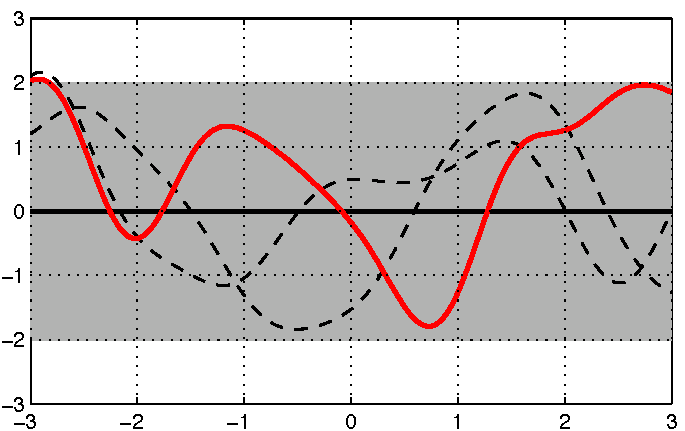
\includegraphics[scale=0.67, clip, trim = 0.5cm 0.45cm 0.2cm 0cm]{figs/gpml/priorGP.pdf}};
	\node at (3.3,-2) {$\bz$};
	\node at (-3.05,1.75) {$\bff(\bz)$};
\end{tikzpicture}
}
\hfill
\subfigure[Samples from the GP posterior $p(\bff|\cD,\hyp)$.]{
\tikzstyle{line} = [draw, -latex]
\begin{tikzpicture}
	\node at (0,0) {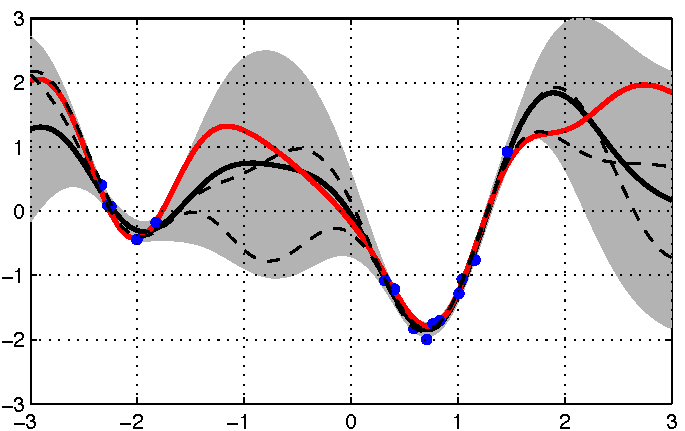
\includegraphics[scale=0.67, clip, trim = 0.5cm 0.45cm 0.2cm 0cm]{figs/gpml/postGP.pdf}};
	\node at (3.3,-2) {$\bz$};
	\node at (-3.05,1.75) {$\bff(\bz)$};
\end{tikzpicture}
\label{fig:post}
}
\caption{Samples from a Gaussian process prior and posterior after data from the underlying function has been observed. The red, black and dashed lines show the underlying function $\bff$, mean of the Gaussian process (prior $\bmm$ and posterior $\bmm_+$) and sampled functions respectively. The grey regions denote two standard deviations, or 95\% confidence region, of the GP distribution. Training data is shown as blue dots on the posterior plot.}
\label{fig:priorpost}
\end{figure}
%-------------------------------------------------------------------------------------------------------------------------------------------


\subsubsection{Posterior}
Given the observed training data set $\cD$ it is desirable to update this prior and form a posterior distribution over the space of functions. This posterior distribution is related to the prior and the training data through Bayes' rule
\begin{equation}
p(\bff|\cD,\hyp) = \frac{p(\bY|\bff,\bZ,\hyp)}{p(\bY|\bZ,\hyp)} p(\bff|\hyp)
\label{eqn:gpbayes}
\end{equation}
with likelihood $p(\bY|\bff,\bZ,\hyp)$ and prior $p(\bff|\hyp)=p(\bff|\bZ,\hyp)$ which is independent of the training inputs. The marginal likelihood term is given by the following equivalent integrals
\begin{align}
p(\bY|\bZ,\hyp) &= \int p(\bY|\bff,\bZ,\hyp)p(\bff|\hyp)\dd\bff 
= \int p(\bY|\bF,\hyp)p(\bF|\bZ,\hyp)\dd\vec\bF
\label{eqn:marlik}
\end{align}
These expressions are equivalent because the observed data set $\bY$ is related to the underlying function $\bff$ only through the underlying values $\bF$ since the likelihood has no notion of the prior beliefs. We shall discuss the importance of this term for training the hyperparameters of a Gaussian process in the following section. Note that the dependence on the structure $\cH$ is assumed implicitly through the hyperparameters. It turns out that this posterior distribution over functions is also a Gaussian process and can be calculated analytically as demonstrated in \Theo{GPpost}. This is again a standard result from the Machine Learning community.






\begin{theo}[Gaussian Process Posterior] \label{theo:GPpost}
Assume that the function $\bff$ has been drawn from some Gaussian process prior $\bff|\hyp \sim \mathcal{GP}(\bO,\bK)$ with hyperparameters $\hyp$ and that the data set $\cD$ given by \Eq{cZY} has been observed. The posterior distribution is also a Gaussian process $\bff|\cD,\hyp \sim \mathcal{GP}(\bmm_+,\bK_+)$ with mean and covariance function
\begin{align}
\bmm_{+}(\bz) &= \bK(\bz,\bZ) \big(\bK_{nn}+\bS_{\be}\otimes\bI\big)^{-1} \vec\bY  \label{eqn:gpmean} \\
\bK_{+}(\bz,\tilde\bz) &= \bK(\bz,\tilde\bz) - 
\bK(\bz,\bZ) \big(\bK_{nn}+\bS_{\be}\otimes\bI\big)^{-1}\bK(\bZ,\tilde\bz) \label{eqn:gpvar}
\end{align}
\espa
\end{theo}

\begin{proof}
Consider the joint distribution of the noisy observed states $\bY$ and the function values $\bff(\bz)$ and $\bff(\tilde\bz)$ to be inferred
\begin{equation}
\left.\bmat{\vec\bY \\ \bff(\bz) \\ \bff(\tilde\bz)} \right| \bz, \tilde\bz, \bZ, \hyp  \sim \cN\left(
\bO,
\bmat{\bK_{nn}+\bS_{\be}\otimes\bI & \bK(\bZ,\bz) & \bK(\bZ,\tilde\bz) \\ 
\bK(\bz,\bZ) & \bK(\bz,\bz) & \bK(\bz,\tilde\bz) \\
\bK(\tilde\bz,\bZ) & \bK(\tilde\bz,\bz) & \bK(\tilde\bz,\tilde\bz)}
\right)
\end{equation}
By conditioning on the observed outputs $\bY$ using the identity for a Gaussian conditional distribution, from \App{gauss}, the result follows.
\qed
\end{proof}

It is clear that this predictive form is exactly the same as was obtained in \Eqs{rbfM2}{rbfV2} by following a parametric approach and extending to possibly infinite dimensional feature spaces using the kernel trick. However in this case the covariance function has been defined directly and there is no need to appeal to a parametric interpretation in terms of a feature vector or a finite set of basis functions.
%
Note that if the covariance function is in the form of a radial basis function, the predictive mean is in the form of a linear sum radial basis functions each centred on a training data point $\bmm_{+}(\bz) = \bK(\bz,\bZ) \bBe$ where $\bBe = \big(\bK_{nn}+\bS_{\be}\otimes\bI\big)^{-1} \vec\bY$.

The process of choosing a prior distribution over function space and forming the posterior based on training data is shown in \Fig{priorpost}. The posterior shown in \Fig{post} clearly shows that in regions where there is a lot of training data the uncertainty in functional predictions reduces significantly whereas in regions with little training data the distribution collapses back to the prior.
Therefore, given an arbitrary state-action pair $\bz_k$, training data set $\cD$ and Gaussian process prior over function space, the predictive distribution over the next state $p(\bx_{k+1}|\bz_k,\cD)$ can be obtained analytically. 








%It is interesting to note that Eq.~(\ref{gpmean}) is in the form of a nominal function of the inputs plus a linear sum of basis functions defined by the covariance function each centred on a point in the training data set
%\begin{align}
%\bm_{\Delta}(\bz_*) &= \bmm(\bz_*) + \bK(\bz_*,\bZ) \bBe
%\end{align}
%where $\bBe = \bK_{\be}^{-1} \big(\vec\bY - \bmm(\bZ)\big) \in \RR^{nE}$ is simply a weighting vector. 


\subsection{Model Selection and Training} \label{sec:nLML}
The preceding section laid out the framework for prediction using a Gaussian process prior with known structural form $\cH$ and hyperparameters $\hyp$. In practice, the form and parameters governing the prior are unknown, and are in fact a construct that has been created in order to view the inference problem from a Bayesian perspective. A fully Bayesian approach to addressing the model selection problem, as outlined in \cite{RaWi06} Chapter 5, can be viewed through the hierarchy depicted by the graphical model in \Fig{modsel}. In this framework a distribution is maintained over hyperparameters and possible model structures as well as the function space itself.

In this thesis, we shall not adopt the fully Bayesian treatment of model selection due to the analytic intractability of integrating over hyperparameter distributions and computational complexity of approximating it using sampling methods. We will assume that the model structure $\cH$ has been chosen beforehand based on intuition about the problem at hand and that a point estimate of the hyperparameters $\hat\hyp$ is chosen based on an evidence maximisation scheme which will now be motivated.

%-------------------------------------------------------------------------------------------------------------------------------------------
\begin{figure}[t]
\centering
%
\tikzstyle{sum} = [circle, draw, minimum height=.8cm]
\tikzstyle{line} = [draw, -latex]
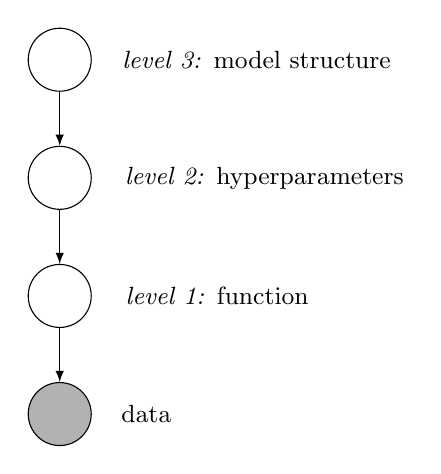
\begin{tikzpicture}
	\node[sum] (H) at (0,2.25) {$\cH$}; \node[sum] (h) at (0,0.75) {$\hyp$};
	\node[sum] (w) at (0,-0.75) {$\bff$}; \node[sum, fill=black!30] (D) at (0,-2.25) {$\cD$};
	\path[line] (H) -- (h); \path[line] (h) -- (w); \path[line] (w) -- (D);
	\node[] at (2.5,2.25) {\small \textit{level 3:} model structure};
	\node[] at (2.6,0.75) {\small \textit{level 2:} hyperparameters};
	\node[] at (2,-0.75) {\small \textit{level 1:} function};
	\node[] at (1.1,-2.25) {\small data};
\end{tikzpicture}
%
\caption{Graphical model depicting the model selection hierarchy from possible model structures $\cH$ to the associated hyperparameters $\hyp$ which in turn control the distribution over the actual underlying function $\bff$ which determines the observed data set $\cD$. The clear nodes depict hidden variables and the gray nodes depict observed variables.}
\label{fig:modsel}
\end{figure}
%-------------------------------------------------------------------------------------------------------------------------------------------

Level 1 inference was discussed in the previous section and is concerned with determining the posterior over function space $p(\bff|\cD,\hyp)$ once a training data set had been observed and given some known hyperparameters. This was achieved using Bayes' rule in \Eq{gpbayes} and it turned out that this could be found analytically in the form of \Eqs{gpmean}{gpvar}.

Level 2 inference considers the distribution over hyperparameters $\hyp$ given a specific model structure $\cH$. The posterior after observing a training data set is again given by Bayes' rule as
\begin{equation}
p(\hyp|\cD) = \frac{p(\bY|\bZ,\hyp)}{p(\bY|\bZ)} p(\hyp) \label{eqn:hypbayes}
\end{equation}
Again, dependence of each term on the model structure is taken implicitly. Now a sensible point estimate for the hyperparameters would be the Maximum A Posteriori (MAP) estimate $\hat\hyp \in \arg\!\max_{\hyp}p(\hyp|\cD)$. Taking a flat prior over hyperparameters means that $p(\hyp|\cD) \propto p(\bY|\bZ,\hyp)$. Therefore maximising the marginal likelihood (or log-marginal likelihood) from \Eq{gpbayes} is equivalent to the MAP estimate of the hyperparameters. This can be written analytically as
\begin{align}
-\log p(\bY|\bZ,\hyp) = 
\underbrace{ \tfrac{1}{2} \big(\vec\bY-\bmm(\bZ)\big)\T \bK_{\be}^{-1} \big(\vec\bY-\bmm(\bZ)\big) }_
{\text{data fit}}
+ \underbrace{\tfrac{1}{2}\log\big|\bK_{\be}\big|}_
{\text{complexity}} + \tfrac{En}{2}\log 2\pi \label{eqn:logmar}
\end{align}
where $\bz \in \RR^D$, $\bK_{\be} = \bK_{nn}+\bS_{\be}\otimes\bI$ since the likelihood $p(\bY|\bF,\bZ,\hyp) = \cN(\vec\bF,\bS_{\be}\otimes\bI)$ and prior $p(\bF|\bZ,\hyp) = \cN\big(\bmm(\bZ), \bK_{nn}\big)$ are simply multivariate Gaussians.

As highlighted in Chapter 5.4 of \cite{RaWi06}, maximising the marginal likelihood leads to some intuitive properties in terms of the trade off between data fit and model complexity. In non-rigorous terms we consider the complexity of a given model to be how quickly the function varies as we move around the $\bz$ space. If the function changes very rapidly then data observed in one region of the $\bz$ space will only be useful for making predictions very close to that region (an exception to this would be if we considered periodic covariance functions). Conversely, if the variations are slow then data observed in one region of the space may be generalised to make predictions in the surrounding regions. 

We shall now provide a crude argument for why the log likelihood in \Eq{logmar} trades off data fit with complexity. Consider a zero mean prior with squared exponential covariance term. As the length scales are increased, the terms in $\bK_{\be}$ become more correlated and therefore the complexity term $\big|\bK_{\be}\big|$ decreases. However at the same time the ``size" of the inverse $\bK_{\be}\inv$ increases and therefore deviations from the prior mean are penalised more heavily. If we maximise the marginal likelihood, we are looking for \textit{the least complex model that explains the data.}





\subsection{Sparse Approximations} \label{sec:sparse}
One of the greatest problems in employing a full Gaussian process model is the computational requirements required as the data set increases. The source of this burden lies mainly in the inversion of the kernel matrix $\bK_{nn}$ and its multiplication with vectors. This issue can be addressed by finding low-rank approximations to this matrix and most of these methods can be viewed under the unifying framework of \cite{QR05}. In this thesis we shall consider the Fully Independent Training Conditional (FITC) approximation (or sparse Gaussian processes using pseudo-inputs) defined by \cite{SG06}. We find this to be a more elegant approach than simply throwing away a subset of the data points.

The FITC approximation assumes that a fictitious (or pseudo) data set $\cD_{\text{p}} = \{\bZ_{\text{p}},\bF_{\text{p}}\}$ of $m<n$ data points is available alongside the actual data $\cD$. Note that it would be meaningless to introduce noise onto the pseudo-targets $\bF_{\text{p}}$ and use $\bY_{\text{p}}$ instead. It turns out that we do not actually need to define values for $\bF_{\text{p}}$ since their effect can be integrated out analytically
\begin{align*}
p(\bY | \bZ, \bZ_{\text{p}}) &= \int p(\bY | \bZ, \bZ_{\text{p}}, \bF_{\text{p}}) p(\bF_{\text{p}} | \bZ_{\text{p}}) \dd \vec{\bF}_{\text{p}} \\
&= \int \cN\big(\vec\bY | \bK_{nm}\bK_{mm}\inv\vec{\bF}_{\text{p}}, \bGam\big) 
\cN\big(\vec{\bF}_{\text{p}} | \bO, \bK_{mm}\big) \dd \vec{\bF}_{\text{p}} \\
&= \cN\big( \vec\bY| \bO, \bQ_{nn} + \bGam \big)
\end{align*}
where $\bK_{nm} := \bK(\bZ,\bZ_{\text{p}})$, $\bK_{mm} := \bK(\bZ_{\text{p}},\bZ_{\text{p}})$ and $\bQ_{nn} := \bK_{nm}\bK_{mm}\inv\bK_{mn}$ is clearly a low rank approximation of $\bK_{nn}$. The matrix $\bGam$ is specific to the FITC approximation and is defined as
\begin{equation*}
\bGam := \diag\{\bK_{nn} - \bQ_{nn}\} + \bS_{\be} \otimes \bI
\end{equation*}
which is distinct from many of the other sparse approximate methods which simply use $\bGam = \bS_{\be} \otimes \bI$. When training, the locations of these pseudo-inputs $\bZ_{\text{p}}$ are optimised along with the hyperparameters $\hyp$.

Now to determine the Gaussian process posterior prediction under this approximation. The posterior mean and covariance are now defined as
\begin{align}
\bmm_{+}(\bz) &= \bK(\bz,\bZ_{\text{p}}) \bB\inv \bK_{mn} \bGam\inv \vec\bY \\
%
\bK_{+}(\bz,\tilde\bz) &= \bK(\bz,\tilde\bz) - \bK(\bz,\bZ_{\text{p}}) \big(\bK_{mm}\inv - \bB\inv\big)\bK(\bZ_{\text{p}},\tilde\bz)
\end{align}
where $\bB := \bK_{mm} + \bK_{mn}\bGam\inv\bK_{nm}$. It is important to note that these equations are in exactly the same form as \Eqs{gpmean}{gpvar} with respect to the test inputs $\bz$ and $\tbz$. This means that employing the FITC sparse approximation will have no effect on our discussion of multiple-step ahead predictions in \Sec{multistep}.





\subsection{Priors for General Nonlinear Functions} \label{sec:kernels}
\subsubsection{Squared Exponential Kernel}

Attention shall now be given to a particular choice of kernel $\bK$, the Squared Exponential (SE). 
To motivate the use of this kernel, consider the single state case where $E=1$. The analysis in the section closely follows that given by \cite{Dei09} in Section 2.2. The standard form of the SE kernel is
\begin{equation}
k_{\text{SE}}(\bz,\tilde\bz) = \alpha^2 \exp\Big(-\tfrac{1}{2}(\bz - \tilde\bz)\T\bLa^{-1}(\bz - \tilde\bz) \Big)
\label{eqn:SEkernel}
\end{equation}
with hyperparameters $\hyp \in \RR^{D+1}$ consisting of an output variance $\alpha^2$ and a diagonal matrix of input length-scales $\bLa = \diag\big\{[\lambda_1^2 \dots \lambda_D^2]\big\}$. \Theo{SEkernel} shows that this kernel defines a prior distribution over the space of all functions in the class of a given universal function approximator.

\begin{theo}[Squared Exponential Kernel] \label{theo:SEkernel}
Consider the function $f:\RR^D \rightarrow \RR$ parameterised by a universal function approximator of the form
\begin{equation}
f(\bz) = \int_{\RR^D}  \phi(\bz,\bs) \gamma(\bs) \dd\bs 
= \int_{\RR^D}  \exp\left( -(\bz-\bs)\T\bLa^{-1}(\bz-\bs) \right)  \gamma(\bs)  \dd\bs
\label{eqn:universalapp}
\end{equation}
where $\gamma(\bs)$ is a weighting function. Assuming a normal Gaussian prior over the weights $\gamma(\bs) \sim \cN(0,1)$ is equivalent to assuming $f \sim \mathcal{GP}(0,k_{\text{SE}})$ has been drawn from a Gaussian process with zero mean and squared exponential covariance function given in \Eq{SEkernel}.
\spa \end{theo}

\begin{proof}
The equivalent Gaussian process representation of this problem will have a mean function given by $\EE_{\gamma}[f(\bz)]$ and covariance function given by $\cov_{\gamma}[f(\bz),f(\tilde\bz)] $. The mean is calculated as
\begin{align*}
\EE_{\gamma}[f(\bz)] &= \int f(\bz) p\big(\gamma(\bs)\big) \dd\gamma(\bs) 
= \int \phi(\bz,\bs) \bigg( \int \gamma(\bs) p\big(\gamma(\bs)\big) \dd\gamma(\bs) \bigg) \dd\bs = 0
\end{align*}
since $\EE_{\gamma}[\gamma(\bs)] = 0$. Now, because the prior mean function equals zero the prior covariance is
\begin{align*}
\cov_{\gamma}[f(\bz),f(\tilde\bz)] &= \EE_{\gamma}[f(\bz)f(\tilde\bz)] \\
&= \int f(\bz) f(\tilde\bz) p\big(\gamma(\bs)\big) \dd\gamma(\bs) \\
&= \int \phi(\bz,\bs) \phi(\tilde\bz,\bs) \bigg( \int \gamma(\bs)^2 p\big(\gamma(\bs)\big) \dd\gamma(\bs) \bigg) \dd\bs \\
&= \int \phi(\bz,\bs) \phi(\tilde\bz,\bs) \dd\bs
\end{align*}
since $\EE_{\gamma}[\gamma(\bs)^2] = 1$. Now because $\phi$ produces an unnormalised Gaussian this integral is tractable and from \Eq{universalapp}
\begin{equation*}
\cov_{\gamma}[f(\bz),f(\tilde\bz)] = \alpha^2 \exp\Big(-\tfrac{1}{2}(\bz - \tilde\bz)\T\bLa^{-1}(\bz - \tilde\bz) \Big)
\end{equation*}
for a suitable $\alpha$. This is exactly the form of the SE kernel in \Eq{SEkernel}.
\qed
\end{proof}

Informally, the SE covariance function provides a means of placing a prior over the space of all smooth, or infinitely differentiable functions, with intrinsic input length scales. 




\subsubsection{Additive Squared Exponential Kernel} 
A related class of kernel functions is the additive squared exponential family. These are useful in the situation where we wish to parameterise a distribution over a space of additively separable functions. The family of first-order additive functions are as follows
\begin{align*}
\bff(\bz) &= \sum_{i=1}^D  \bff_i\big(z[i]\big)
\end{align*}
We may also wish to consider higher order interaction terms.
We shall consider a general additive form in which the orders of interaction are stored in the set $\cI$ and can be written mathematically as
\begin{align}
\bff(\bz) &= \sum_{\bi \in \cI}  \bff_\bi\big(\bz[\bi]\big)
\end{align}
For example if we know our function is an additive combination of nonlinear functions with respect to the first, third and a combination of the second and third components of the state-action space then $\cI = \{1,3,[2;3]\}$. Considering $D\tth$ order interactions $\cI = \{[1 \dots D]\}$ will obviously brings us back to the completely general function $\bff(\bz)$. 
%
Now a kernel that parameterises a prior distribution over such a space is the additive squared exponential which we define as follows
\begin{equation}
k_{\text{aSE}}(\bz,\tilde\bz) = \sum_{\bi \in \cI} \alpha_{\bi}^2 \exp\Big(-\tfrac{1}{2}\big(\bz[\bi] - \tilde\bz[\bi]\big)\T\bLa_{\bi}^{-1}\big(\bz[\bi] - \tilde\bz[\bi]\big) \Big)
\label{eqn:aSEkernel}
\end{equation}
where it is clear that setting $\cI = \{[1 \dots D]\T\}$ recovers the standard squared exponential kernel.

In the literature the first order additive structure appears under Generalized Additive Models (GAMs) as introduced by \cite{HT90}. The general kernel involving all possible interactions was recently introduced by \cite{DNR11}. The authors attack the main drawback this general kernel, which is the computational effort required to calculate all the terms, which scales as $\cO(2^n)$. They present a neat iterative method of evaluating all the additive kernels in $\cO(D^2)$ making it a useful and computationally tractable model to work with. This method requires that the $\alpha_{\bi}$ and $\bLa_\bi$ parameters are common for each order of interaction, which is not too restrictive. It is based on the Newton-Girard formulae, which assumes that the function can be decomposed as a product
\begin{equation*}
k_{\text{aSE}}(\bz,\tilde\bz) = \sum_{\bi \in \cI} \alpha_{\bi}^2 \prod_{i\in \bi} \exp\Big(-\tfrac{1}{2}\big(z[i] - \tilde z[i]\big)^2/\lambda_{i}^{2} \Big)
\end{equation*}
As we shall see in \Sec{multistep} this decomposable structure is lost when we are considering prediction at an uncertain state-input and therefore this iterative method cannot be used. Therefore for most applications we will only be considering separating first order, and maybe second order, interactions and leaving higher order ones to be explained by a standard SE kernel.







\section{Multiple-Step Predictions} \label{sec:multistep}
\subsection{Overview}
A framework for maintaining a Gaussian distribution over whole trajectories $\btau$ based on a moment matching approximation was outlined in \Sec{xuprediction}. In order for a Gaussian process model to fit into this framework the mean $\bmm$ and covariance function $\bK$ must be of a form such that the expectation $\bm_* = \EE_{\bz,\bff}[\bff(\bz)]$ and covariance $\bS_* = \cov_{\bz,\bff}[\bff(\bz)]$ are analytically tractable given $\bff\sim\mathcal{GP}(\bmm_+,\bK_+)$ and $\bz \sim \cN(\bm,\bS)$. The posterior mean $\bmm_+$ and covariance $\bK_+$ are related to the input mean $\bm$ and covariance $\bS$ through the GP predictive equations given in \Eqs{gpmean}{gpvar}. Through separation of the integrals with respect to the random function $\bff$ and the input $\bz$ the expectation, covariance and output-input covariance can be broken down as follows
\begin{align}
\bm_* &=  \EE_{\bz,\bff}[\bff(\bz)]
&& \!\!\!\!\!\!\!\!\!\!\!\!\!\!\!\!\!\!\!\!\!\!\!\!\!\!\!\!\!\!\!\!\!\!\!\!\!\!\!\!\!\!\!\!\!\!\!\!\!
= \EE_{\bz}[\bmm_+(\bz)] \label{eqn:uncM} \\
\bS_* &= \cov_{\bz,\bff}[\bff(\bz)] 
&& \!\!\!\!\!\!\!\!\!\!\!\!\!\!\!\!\!\!\!\!\!\!\!\!\!\!\!\!\!\!\!\!\!\!\!\!\!\!\!\!\!\!\!\!\!\!\!\!\!
= \EE_{\bz}\big[\bK_+(\bz) + \bmm_+(\bz)\bmm_+(\bz)\T\big] - \bm_*\bm_*\T \label{eqn:uncV} 
\end{align}
An example of the moment matching approximation for the posterior GP shown in \Fig{post} is given in \Fig{multiprop}. The exact expressions for these equations shall now be derived for a linear mean function along with a linear, squared exponential or additive squared exponential covariance function.







%-------------------------------------------------------------------------------------------------------------------------------------------
\begin{figure}[t]
\centering
\small
\tikzstyle{line} = [draw, -latex]
\begin{tikzpicture}
\node at (0,-3) {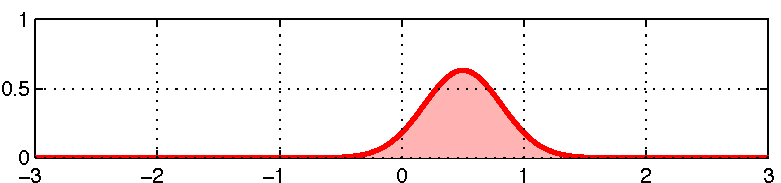
\includegraphics[scale=0.6, clip, trim=0.5cm 0.3cm 0cm 0cm]{figs/gpml/propGP_1.pdf}};
\node at (0.025,0) {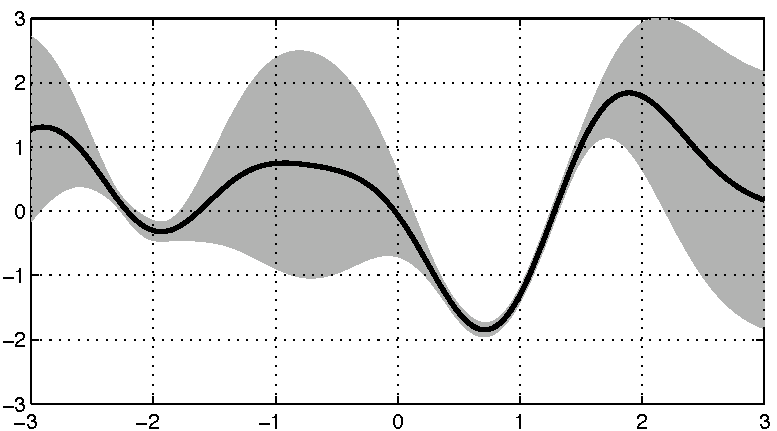
\includegraphics[scale=0.6, clip, trim=0.5cm 0.4cm 0cm 0cm]{figs/gpml/propGP_2.pdf}};
\node at (4.7,0) {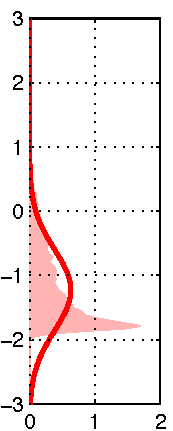
\includegraphics[scale=0.6, clip, trim=0.45cm 0.4cm 0cm 0cm]{figs/gpml/propGP_3.pdf}};

\node[rotate=90] at (-4.13,0) {Gaussian process};
\node[rotate=-90] at (5.65,0) {\color{red}Output distribution};
\node at (0,-4.1) {\color{red}Input distribution};

\node at (-3.1,1.55) {$p(\bff)$};
\node at (-3.1,-2.7) {\color{red}$p(\bz)$};
\node at (4.7,1.55) {\color{red}$p\big(\bff(\bz)\big)$};

\end{tikzpicture}
\caption{The moment matching approximation for a Gaussian process evaluated at a distribution over state-actions $p(\bz)$. The red lines depict the Gaussian approximations to the true distributions given by the red shaded areas.}
\label{fig:multiprop}
\end{figure}
%-------------------------------------------------------------------------------------------------------------------------------------------





\subsection{Parametric Form}
\subsubsection{General Basis Functions}
We shall first consider the predictive equations $\bmm_+(\bz)$ and $\bK_+(\bz)$ for a parametric model consisting of a linear sum of known basis functions as given in \Eqs{rbfM}{rbfV}. Remember that this approach can be viewed from a function space perspective as a Gaussian process for which there exists a finite inner product representation of the covariance function $\bK(\bz,\tilde\bz) = \bPh(\bz)\T\bOm\bPh(\tilde\bz)$. 
%
The elements of the terms in \Eqs{uncM}{uncV} are given by 
\begin{align*}
\mu_{*}[i] &= 
\EE_{\bz}\big[\bph_{i}\big]\T \bet_{+} \\
%
\Sigma_{*}[i,j] &= 
\tr\Big(\EE_{\bz}\big[\bph_{i}\bph_{j}\T\big] \big(\bOm_{+}+\bet_+\bet_+\T\big) \Big) 
- \mu_{*}[i]\mu_{*}[j]
\end{align*}
for $i,j \in \ZZ_{[1,E]}$ where $\bph_{i} = \Phi[:,i](\bz)$. 
%
With the use of the Kronecker and Hadammard products we can actually define an expression for the full mean $\bm_*$ and covariance $\bS_*$ as follows
\begin{align}
\bm_* &= (\bI_E \otimes \mathbf{1}_P\T) \Big( \EE_{\bz}\big[\vec{\bPh}\big] \circ \big(\mathbf{1}_E \otimes \bet \big) \Big)
 \label{eqn:uncparamM}  \\
%
\bS_* &= 
 (\bI_E \otimes \mathbf{1}_P\T)
\Big( \EE_{\bz}\big[\vec{\bPh}\vec{\bPh}\T\big]  \circ 
\big(\mathbf{1}_{E\times E} \otimes (\bOm+\bet\bet\T) \big) \Big) 
 (\bI_E \otimes \mathbf{1}_P)
- \bm_*\bm_*\T
\label{eqn:uncparamV}
\end{align}
where $\vec{\bPh} = \vect\big(\bPh(\bz)\big)$. Note that the $(\bI_E \otimes \mathbf{1}_P)$ terms act as a kind of multivariable trace operator in the expression for $\bS_*$. We could not find this form anywhere in the literature and therefore the derivation of it is our own.
%
This expression means that the only requirement on the feature matrix is that the expectations $\EE_{\bz}\big[\vec{\bPh}]$ and $\EE_{\bz}\big[\vec{\bPh}\vec{\bPh}\T\big]$ can be evaluated analytically.





\subsubsection{Linear Model}
For the standard linear model the feature matrix is given by $\bPh(\bz) = \bI \otimes \bz$, \Eqs{uncparamM}{uncparamV} take the following simplified form
\begin{align}
\bm_* &= (\bI_E \otimes \mathbf{1}_D\T) \Big( \big( \mathbf{1}_E \otimes \EE_{\bz}[\bz] \big) \circ \bet \Big) 
\label{eqn:linMU} \\
%
\bS_* &= 
 (\bI_E \otimes \mathbf{1}_D\T)
\Big( \big(\mathbf{1}_{E\times E} \otimes \EE_{\bz}\big[\bz\bz\T\big] \big) \circ 
 \big(\bOm+\bet\bet\T\big) \Big) 
 (\bI_E \otimes \mathbf{1}_D)
- \bm_*\bm_*\T
\label{eqn:linSIG}
\end{align}








\subsection{Nonparametric Form}

\subsubsection{General Covariance Function}
We now turn our attention back to the more general nonparametric form of these equations. Consider the standard Gaussian process predictive equations given in \Eqs{gpmean}{gpvar}. The elements of the predictive equations in \Eqs{uncM}{uncV} are given by 
%%
\begin{align*}
\mu_*[i] &= 
\EE_{\bz}\big[\bk_{i}\big]\T \bBe \\
%
\Sigma_*[i,j] &= 
\EE_{\bz}\big[k_{ij}\big] + \tr\Big(\EE_{\bz}\big[\bk_{i}\bk_{j}\T\big]
\big(\bK_{\be}^{-1} + \bBe\bBe\T\big) \Big) 
- \mu^{(i)}_* \mu^{(j)}_*
\end{align*}
%%
for $i,j \in \ZZ_{[1,E]}$ where $\bk_{i} = K[:,i](\bZ,\bz)$ is the $i\tth$ column of $\bK(\bZ,\bz)$ and $k_{ij}=K[i,j](\bz)$ is the $(i,j)\tth$ element of $\bK(\bz)$. 
Note that if we are employing a sparse GP approximation then we simply replace the vector $\bBe$ and matrix $\bK_{\be}$ with the appropriate terms and the rest of the analysis remains the same.
Now, as with the parametric form, expressions may be written for the full mean and covariance as follows
%%
\begin{align}
\bm_* &= (\bI_E \otimes \mathbf{1}_n\T)
\Big( \EE_{\bz}\big[\vec{\bK}\big] \circ \big(\mathbf{1}_E \otimes \bBe \big) \Big)
 \label{eqn:uncgpM}  \\
%
\bS_* &= 
\EE_\bz[\bK(\bz)] + 
 (\bI_E \otimes \mathbf{1}_n\T)
\Big( \EE_{\bz}\big[\vec{\bK}\vec{\bK}\T\big]  \circ 
\big(\mathbf{1}_{E\times E} \otimes (\bK_{\be}^{-1} + \bBe\bBe\T) \big) \Big) 
 (\bI_E \otimes \mathbf{1}_P)
- \bm_*\bm_*\T
\label{eqn:uncgpV}
\end{align}
%%
where $\vec{\bK} = \vect\big( \bK(\bZ,\bz) \big)$. Again, this is a novel parameterisation that has not been found in the literature.
%
Similarly to the parametric form, the only requirements on the covariance function is that the expectations $\EE_{\bz}\big[\bK(\bz)\big]$, $\EE_{\bz}\big[\vec{\bK}\big]$ and $\EE_{\bz}\big[\vec{\bK}\vec{\bK}\T\big]$ are analytically tractable. In most cases, stationary covariance functions will be considered i.e.\ $\bK(\bz,\tilde\bz) = \bK(\bz-\tilde\bz)$ therefore $\bK(\bz)$ will be a constant matrix. The remaining expectations will be made up of the building blocks
\begin{align}
\EE_{\bz}\big[ k_a(\ba,\bz) \big] \quad \text{and} \quad
\EE_{\bz}\big[ k_a(\ba,\bz)k_b(\bb,\bz) \big] \label{eqn:exps}
\end{align}
where $k_a(\ba,\bz)$ and $k_b(\bb,\bz)$ are elements of $\bK(\ba,\bz)$ and $\bK(\bb,\bz)$ respectively and $\ba,\bb \in \bZ$. We will now evaluate these expectations for the squared exponential kernel.







\subsubsection{Squared-Exponential Kernel} 
The following derivations can be found in \cite{Dei09}, Section 2.3 or \cite{GRQM03} for the univariate case. Consider the squared exponential kernel defined in \Eq{SEkernel}. The first expectation in \Eq{exps} can then be expanded as
\begin{align}
\nonumber \EE_{\bz}\big[ k_a(\ba,\bz) \big] 
&= \int k_a(\ba,\bz) \cN(\bz|\bm,\bS) \dd\bz \\
\nonumber &= \alpha_a^2(2\pi)^{\sfrac{D}{2}} |\bLa_a|^{\sha}  \int  \cN(\bz|\ba,\bLa_a) \cN(\bz|\bm,\bS)  \dd\bz   \\[-0.3cm]
\nonumber &= \alpha_a^2 (2\pi)^{\sfrac{D}{2}} |\bLa_a|^{\sha} \cN\big(\bm|\ba,\bLa_a+\bS\big) 
\overbrace{ \int \cN\big(\bz|\bm_{\ba},\bS_{\ba} \big)  \dd\bz }^{ 1 }   \\
&=  \alpha_a^2  \big|\bS\bLa_a\inv + \bI\big|^{-\sha} \exp\Big( -\half(\ba-\bm)\T(\bLa_a+\bS)\inv (\ba-\bm)\Big) 
\label{eqn:SEpropM}
\end{align}
The first step is made by pulling out the normalising constant for the squared exponential kernel to make it a Gaussian and the second step is due to the identity for the multiplication of two Gaussian densities given in \App{gauss}. Note that setting $\bS = \sigma\bI$ and letting $\sigma \rightarrow 0$, the standard expression for the SE kernel is recovered as expected. The mean $\bm_{\ba}$ and covariance $\bS_{\ba}$ are given by
\begin{align}
\bm_{\ba} &:= (\bLa_a\inv + \bS\inv)\inv \big(\bLa_a\inv\ba + \bS\inv\bm \big)
&&\!\!\!\!\!\!\!\!\!\!\!\!\!\!\!\!\!\!\!\!\!\!\!\!\!\!\!\!\!\!\!\!\!=  (\bS\bLa_a\inv + \bI)\inv \big( \bS\bLa_a\inv\ba + \bm \big)
\label{eqn:muA} \\
\bS_{\ba} &:= (\bLa_a\inv + \bS\inv)\inv
&&\!\!\!\!\!\!\!\!\!\!\!\!\!\!\!\!\!\!\!\!\!\!\!\!\!\!\!\!\!\!\!\!\!= (\bS\bLa_a\inv + \bI)\inv \bS
\label{eqn:sigA}
\end{align}
which can be written in a form in which there is no need to invert the potentially singular matrix $\bS$ explicitly.
Now turning to the second expectation in \Eq{exps} and following a similar procedure gives
\begin{align*}
\EE_{\bz}[k_a(\ba,\bz)&k_b(\bb,\bz)\big] \\
&= \int k_a(\ba,\bz)k_b(\bb,\bz) \cN(\bz|\bm, \bS) \dd\bz \\
%
&= \alpha_a^2\alpha_b^2 (2\pi)^{D} |\bLa_a|^{\sha} |\bLa_b|^{\sha}
\int \cN(\bz|\ba,\bLa_a)\cN(\bz|\bb,\bLa_b) \cN(\bz|\bm, \bS) \dd\bz  \\[-0.3cm]
%
&= \alpha_a^2\alpha_b^2 (2\pi)^{D} |\bLa_a|^{\sha} |\bLa_b|^{\sha}
\cN\big(\ba|\bb,\bLa_a+\bLa_b\big) \cN\big(\bm|\hat\bm,\hat\bS \big)
\overbrace{ \int \cN(\bz|\bm_{\ba\bb},\bS_{\ba\bb}) \dd\bz }^{ 1 } \\
%
&= \alpha_a^2 \alpha_b^2 \big|\bS(\bLa_a\inv + \bLa_b\inv) + \bI\big|^{-\sha}
\exp\Big( -\half(\ba-\bb)\T(\bLa_a + \bLa_b)\inv (\ba-\bb) \Big) \\
&\quad\quad\quad\quad\quad\quad\quad\quad\quad\quad\quad\quad\quad\quad\quad\quad\quad\quad
 \exp\Big( -\half(\hat\bm-\bm)\T(\hat\bS + \bS)\inv (\hat\bm-\bm) \Big)
\end{align*}
where $\hat\bm := \hat\bS(\bLa_a\inv\ba + \bLa_b\inv\bb)$ and $\hat\bS := (\bLa_a\inv + \bLa_b\inv)\inv$. This can be written in a more intuitive manner by expanding and collecting terms in the exponents
%
\begin{equation}
\EE_{\bz}[k_a(\ba,\bz)k_b(\bb,\bz)\big] = k_a(\ba,\bm)k_b(\bb,\bm) \big|\bR\big|^{-\sha}
\exp\Big( \half\bar\bm\T \bR\inv\bS \bar\bm \Big)
\label{eqn:SEpropV}
\end{equation}
%
where $\bR := \bS(\bLa_a\inv+\bLa_b\inv) + \bI$ and $\bar\bm := \bLa_a\inv(\ba-\bm) + \bLa_b\inv(\bb-\bm)$. Note that $\bR\inv\bS = (\bLa_a\inv+\bLa_b\inv + \bS\inv)\inv$ is a symmetric matrix and can again be computed without explicit inversion of $\bS$. For completeness, note that the mean $\bm_{\ba\bb}$ and covariance $\bS_{\ba\bb}$ are given by
\begin{align}
\bm_{\ba\bb} &:= (\bLa_a\inv + \bLa_b\inv + \bS\inv)\inv \big(\bLa_a\inv\ba + \bLa_b\inv\bb + \bS\inv\bm \big)
&&\!\!\!\!\!\!=  \bR\inv \big( \bS(\bLa_a\inv\ba + \bLa_b\inv\bb) + \bm \big)
\label{eqn:muAB} \\
\bS_{\ba\bb} &:= (\bLa_a\inv + \bLa_b\inv + \bS\inv)\inv
&&\!\!\!\!\!\!= \bR\inv \bS
\label{eqn:sigAB}
\end{align}
To conclude, the expectations required for moment matching in \Eq{exps} are given by \Eqs{SEpropM}{SEpropV} for the squared exponential kernel defined in \Eq{SEkernel}.



\subsubsection{Additive Squared-Exponential Kernel} 
The following derivations are new to the field and a contribution of our work. The key to deriving these equations comes from the observation that an infinite length scale associated with a variable is equivalent to ignoring it. This means that we can re-write the additive kernel defined in \Eq{aSEkernel} as
\begin{equation}
k(\bz,\tilde\bz) = \sum_{\bi \in \cI} \alpha_{\bi}^2 
\exp\Big(-\tfrac{1}{2}
\big(\bz - \tilde\bz\big)\T  \bXi_{\bi}^{-1}  
\big(\bz - \tilde\bz\big) \Big)
\end{equation}
where $\bXi_\bi\inv \in \RR^{D\times D}$ is a diagonal matrix with nonzero elements given by the diagonal of $\bLa_\bi\inv$ on the appropriate dimension. For example if $D=3$, $\bi = [1;3]$ and $\bLa_\bi\inv = \diag\{[\lambda_1^{-2}, \lambda_3^{-2}]\}$ then $\bXi_\bi\inv = \diag\{[\lambda_1^{-2}, 0, \lambda_3^{-2}]\}$. Acknowledging this means that we can derive the appropriate equations directly from the SE equations in \Eqs{SEpropM}{SEpropV}. The first expectation is
%
\begin{align}
\nonumber \EE_{\bz}\big[ &k_a(\ba,\bz) \big] \\
\nonumber &=  \sum_{\bi \in \cI} \alpha_{\bi a}^2  \big|\bS\bXi_{\bi a}\inv + \bI\big|^{-\sha} \exp\Big( -\half(\ba-\bm)\T(\bXi_{\bi a}+\bS)\inv (\ba-\bm)\Big) \\
%
&=  \sum_{\bi \in \cI} \alpha_{\bi a}^2  \big|\bS[\bi,\bi]\bLa_{\bi a}\inv + \bI\big|^{-\sha}
\exp\Big( -\half\big(\ba[\bi]-\bm[\bi]\big)\T\big(\bLa_{\bi a}+\bS[\bi,\bi]\big)\inv \big(\ba[\bi]-\bm[\bi]\big)\Big) 
\label{eqn:aSEpropM}
\end{align}
while the second is 
\begin{equation}
\EE_{\bz}[k_a(\ba,\bz)k_b(\bb,\bz)\big] = \sum_{\bi \in \cI}\sum_{\bj \in \cI}k_a(\ba,\bm)k_b(\bb,\bm) \big|\bR_{\bi\bj}\big|^{-\sha}
\exp\Big( \half\bar\bm\T \bR_{\bi\bj}\inv\bS \bar\bm \Big)
\label{eqn:aSEpropV}
\end{equation}
where $\bR_{\bi\bj} := \bS(\bXi_{\bi a}\inv+\bXi_{\bj b}\inv) + \bI$ and $\bar\bm := \bXi_{\bi a}\inv(\ba-\bm) + \bXi_{\bj b}\inv(\bb-\bm)$. Observe that all $\bXi$ variables appear in their inverted form while $\bS$ appears only as itself which means that calculation of these terms can be done in a numerically stable manner. 




\section{Constraints}
\subsection{State Constraints}


It should be noted that the following general manner in which to address state and action constraints is a further contribution of this thesis. First, observe that the optimisation problem posed in \Eqs{learn1}{learn2} is unconstrained. However, state and action constraints can still be addressed.
Consider the case where the state is constrained to lie within some convex polytope $\XX = \big\{\bx \in \RR^E \big| \bG\bx + \bg \in [-\mathbf{1},\mathbf{1}] \big\}$ parameterised by $\bG \in \RR^{G\times E}$ and $\bg \in \RR^{G}$. This can be addressed in the probabilistic framework by soft constraints implemented using barrier functions. Two examples of functions for which the expectation with respect to $\bx \sim \cN$ can be evaluated analytically are polynomial and affine barrier functions
\begin{align}
c_{\text{poly}}(\bx) &= \sum_{i=1}^G \Big( g_i(\bx) \Big)^p
\label{eqn:con_poly} \\
c_{\text{aff}}(\bx) &= \sum_{i=1}^G \left\{\begin{matrix}[cc]
-m\Big(g_i(\bx) + 1\Big) & \!\!\!\!\!\!\!\!\!\!\!\!\!\! \text{if } g_i(\bx) \leq -1 \\
0 &  \text{if } -1 < g_i(\bx) \leq 1 \\
m\Big(g_i(\bx) - 1\Big) & \!\!\!\!\!\!\!\!\!\!\!\!\!\!\!\!\!\! \text{if } g_i(\bx) > 1
\end{matrix} \right.
\label{eqn:con_aff}
\end{align}
where $g_i(\bx) = \bG^{(i,:)}\bx + g^{(i)}$, $p$ is the order of the polynomial and $m$ is the gradient of the slope. These are depicted in \Fig{cost_barriers}. Note that the traditional log-barrier function is inappropriate in this context since the integral with respect to a Gaussian would be infinite.



%-------------------------------------------------------------------------------------------------------------------------------------------
\begin{figure}
\centering
\tikzstyle{line} = [draw, -latex]
\begin{tikzpicture}
\small
\node at (0,0) {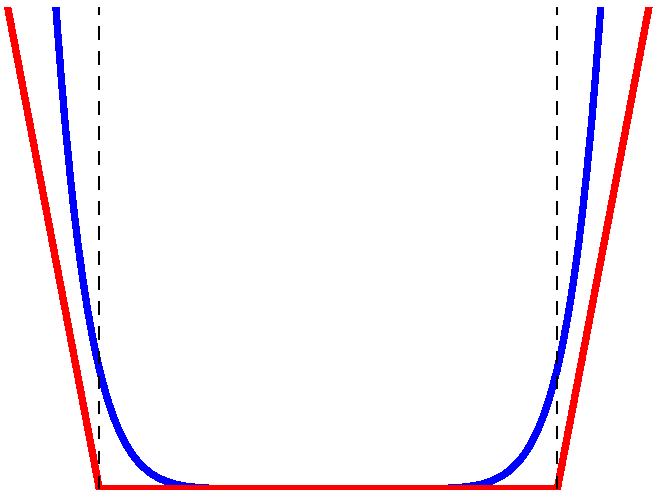
\includegraphics[scale=0.45]{figs/gpml/cost_barriers.pdf}};
\path[line] (-3.5,-1.95) -- (-3.5,2.2);
\path[line] (-3.6,-1.85) -- (3.6,-1.85);
\node at (3.5,-2.1) {$x$};
\node at (-1.5,-2.1) {$x_{\text{min}}$};
\node at (-3.0,2.1) {$c(x)$};
\node at (2,-2.1) {$x_{\text{max}}$};

\draw[dashed] (-3.5,-0.95) -- (3.4,-0.95);
\node at (-3.8,-0.95) {1};
\end{tikzpicture}
\caption{Barrier functions for which the expectation in \Eq{costint} can be evaluated analytically for $x \sim \cN$. These functions in are useful for penalising deviations outside of the set defined by $x_{\min}$ and $x_{\max}$. The polynomial is shown in blue and the affine is shown in red.}
\label{fig:cost_barriers}
\end{figure}
%-------------------------------------------------------------------------------------------------------------------------------------------


\subsection{Action Constraints} \label{sec:actioncon}

Constraints on the action space, again in the form of a convex polytope $\UU = \big\{\bu \in \RR^F \big| \bH\bu + \bh \in [-\mathbf{1},\mathbf{1}] \big\}$ parameterised by matrix $\bH \in \RR^{H\times F}$, can be addressed directly through the way in which the policy $\bpi$ is structured. Note that in this section $H$ shall denote the number of action constraints rather than the prediction horizon. A policy $\bpi: \RR^{E} \rightarrow \UU$ can be constructed in the following general form for $H \geq F$ linearly independent constraints
\begin{equation}
\bpi(\bx) = \bH^{\dagger} \mathrm{\mathbf{sat}}\big( \bH\tilde\bpi(\bx) + \bh \big) - \bH^{\dagger}\bh
\end{equation}
where $\bH^{\dagger} = (\bH\T\bH)\inv\bH\T$ is the right pseudo-inverse of $\bH$ and $\tilde\bpi: \RR^{E} \rightarrow \RR^F$ is a general unconstrained policy structure. The saturation function $\mathrm{\mathbf{sat}}: \RR^{H} \rightarrow \RR^{H}$ has elements
\begin{equation}
\mathrm{sat}^{(i)}(\bu) = \left\{ \begin{matrix}
-1 & \!\!\!\!\!\!\!\!\!\!\!\!\!\! \text{if } u^{(i)} \leq -1 \\
u^{(i)} & \text{if } -1 < u^{(i)} \leq 1 \\
1 & \!\!\!\!\!\!\!\!\!\!\!\!\!\!\!\!\!\! \text{if } u^{(i)} > 1
\end{matrix} \right.
\end{equation}
for $i \in \ZZ_{[1,H]}$. However, this will not fit into the moment matching framework since $\cov_{\bu}[\mathrm{\mathbf{sat}}(\bu)]$ for $\bu \sim \cN$ cannot be evaluated in closed form. Therefore this function is approximated using sinusoids, for which moment matching is possible. Two candidate approximations are
\begin{align}
s_1(u) &= \sin(u) \label{eqn:gsin} \\
s_2(u) &= \tfrac{9}{8}\sin\big(\tfrac{2}{3}u\big) + \tfrac{1}{8}\sin(2u) \label{eqn:gsat}
\end{align}
which are depicted in \Fig{sinsat}. Note that a standard Fourier series expansion would not be appropriate since the approximation must lie in the closed region $s_i(u) \in [-1,1]$ and have unit gradient at the origin $s'_i(0) = 1$ such that $\bpi(\bx) \approx \tilde\bpi(\bx)$ for $\bH\tilde\bpi(\bx) + \bh \approx \bO$. Again, defining the action constraints in this general way is also a contribution of this thesis.


%-------------------------------------------------------------------------------------------------------------------------------------------
\begin{figure}[t]
\centering
%
\tikzstyle{line} = [draw, -latex]
\begin{tikzpicture}
	\small
	\node at (0,0) {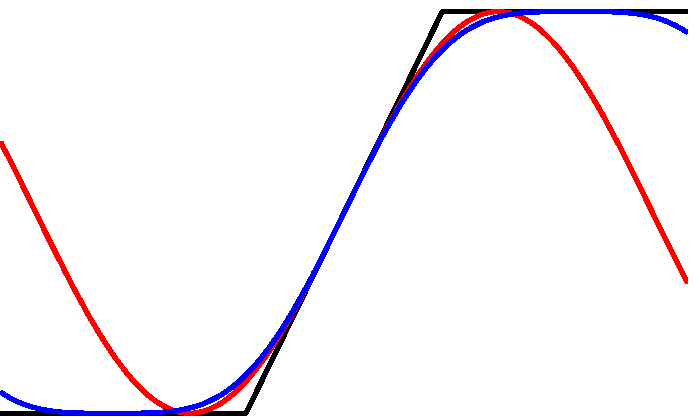
\includegraphics[scale=0.6]{figs/gpml/saturation.pdf}};
	\path[line] (0,-2.3) -- (0,2.3); \path[line] (-4,0) -- (4,0);
	\node at (3.8,-0.3) {$u$};
	\node at (3.8,2.3) {$\mathrm{sat}(u)$};
	\node at (3.8,1.5) {\color{blue}$s_2(u)$};
	\node at (3.8,-1) {\color{red}$s_1(u)$};
	
	\draw[dashed] (0.95,0) -- (0.95,2); \draw[dashed] (0,2) -- (0.95,2);
	\node at (0.95,-0.3) {1}; \node at (-0.3,2) {1};
	\draw[dashed] (-1.05,0) -- (-1.05,-2.07); \draw[dashed] (0,-2.07) -- (-1.1,-2.07);
	\node[fill=white] at (-1.05,-0.3) {-1}; \node[fill=white] at (-0.3,-2.07) {-1};
\end{tikzpicture}
%
\caption{Approximations to the $\mathrm{sat}$ function for which the expectation and covariance with respect to a Gaussian distributed input can be evaluated analytically. Specifically $s_1(u) = \sin(u)$ and $s_2(u) = \tfrac{9}{8}\sin\big(\tfrac{2}{3}u\big) + \tfrac{1}{8}\sin(2u)$. Both satisfy the conditions $s_i(u) \in [-1,1]$ and $s'_i(0) = 1$.}
\label{fig:sinsat}
\end{figure}
%-------------------------------------------------------------------------------------------------------------------------------------------


\section{Summary}
In this chapter we have defined the learning control framework, based on the algorithm of \cite{DR11}, that we shall use in the remainder of this thesis. We have outlined how Gaussian processes can be used as a probabilistic modelling tool for dynamical systems and how they can be used to obtain distributions over full trajectories in the state-action space. Kernels that can be used for defining distributions over linear systems, general additive systems and nonlinear systems have also been introduced. Finally, methods for handling state and action constraints have been given.

